\documentclass[conference]{IEEEtran}
\IEEEoverridecommandlockouts
% The preceding line is only needed to identify funding in the first footnote. If that is unneeded, please comment it out.
\usepackage{cite}
\usepackage{amsmath,amssymb,amsfonts}
% \usepackage{algorithmic}
\usepackage{graphicx}
\usepackage{textcomp}
\usepackage{xcolor}
\usepackage{natbib}
\usepackage[utf8]{inputenc} % allow utf-8 input
\usepackage[T1]{fontenc}    % use 8-bit T1 fonts
\usepackage{hyperref}       % hyperlinks
\usepackage{url}            % simple URL typesetting
\usepackage{booktabs}       % professional-quality tables
\usepackage{amsfonts}       % blackboard math symbols
\usepackage{nicefrac}       % compact symbols for 1/2, etc.
\usepackage{microtype}      % microtypography
\usepackage{xcolor}         % colors
\usepackage{amsmath}
\usepackage{amssymb}
\usepackage{mathtools}
\usepackage{amsthm}
\usepackage{tabularx}
\usepackage{changepage}
% if you use cleveref..
\usepackage[capitalize,noabbrev]{cleveref}
\usepackage{graphicx}
\usepackage{multirow}
% \usepackage{subfigure}
\usepackage{booktabs} % for professional tables
\usepackage{threeparttable}
\usepackage{algorithm}
\usepackage{algpseudocode}
\usepackage{adjustbox}
\usepackage{enumitem}
% \usepackage{subfigure}
\usepackage[caption=false]{subfig}
% \usepackage[caption=false,font=footnotesize]{subcaption}
\def\BibTeX{{\rm B\kern-.05em{\sc i\kern-.025em b}\kern-.08em
    T\kern-.1667em\lower.7ex\hbox{E}\kern-.125emX}}
\begin{document}


\title{\textit{DenoiseRep\textsuperscript{++}}: Enhanced Denoising Model for\\ Representation Learning\\}


\author{Guan'an~Wang$^{\dagger}$,
        Zhengrui~Xu$^{\dagger}$,
        Xiaowen~Huang$^{\ast}$,
        % Jitao~Sang, \\
        Zengguang Hou,\\
        Shaogang Gong,
        Jian Zhang,
        Jitao~Sang
\thanks{Guan’an Wang is an independent researcher (email: guan.wang0706@gmail.com).}%
\thanks{Zhengrui Xu, Xiaowen Huang and Jitao Sang are with the School of Computer Science and Technology, Beijing Jiaotong University (email: {zrxu430; xwhuang; jtsang}@bjtu.edu.cn).}%
\thanks{Xiaowen Huang and Jitao Sang are also with the Beijing Key Laboratory of Traffic Data Mining and Embodied Intelligence, and with the Key Laboratory of Big Data \& Artificial Intelligence in Transportation, Ministry of Education.}%
\thanks{Zengguang Hou is with State Key Laboratory of Multimodal Artificial Intelligence Systems, Institute of Automation, Chinese Academy of Sciences (zengguang.hou@ia.ac.cn).}%
\thanks{Shaogang Gong is with the School of Electronic Engineering and Computer Science, Queen Mary University of London, UK (e-mail: s.gong@qmul.ac.uk).}%
\thanks{Jian Zhang is with the School of Electronic and Computer Engineering, Peking University, China (e-mail: zhangjian.sz@pku.edu.cn).}%
\thanks{$^\dagger$These authors contributed equally to this work.}%
\thanks{$^\ast$Corresponding author.}%
}


\maketitle

\begin{abstract}
The denoising model has demonstrated remarkable capability as a generative framework, yet its potential in discriminative tasks remains underexplored.
%
Representation learning plays a key role in such discriminative settings, which can be defined as \textit{"the process of learning data representations (or features) that facilitate the extraction of meaningful information for building classifiers or other predictive models"}~\cite{6472238}.
%
In this work, we introduce a new approach, termed Enhanced Denoising Model for Representation Learning (\textit{DenoiseRep\textsuperscript{++}}), which jointly performs feature extraction and denoising to enhance feature discriminability.
%
In \textit{DenoiseRep\textsuperscript{++}}, every embedding layer of the backbone network is interpreted as a denoising layer, enabling recursive refinement of representations layer by layer. This design conceptually bridges the two processes—feature extraction, which hierarchically embeds representations from shallow to deep levels, and denoising, which progressively removes noise through successive stages.
%
Subsequently, \textit{DenoiseRep\textsuperscript{++}} merges the parameters of feature extraction and denoising modules, and \textit{theoretically proves} that the pre- and post-fusion forms are mathematically equivalent, thereby eliminating additional computational cost for denoising.
%
Moreover, we extend \textit{DenoiseRep\textsuperscript{++}} with two synergistic enhancements. (1) To enhance the representational capacity of the denoising module, we employ a more expressive teacher network during training for
knowledge distillation. Specifically, the teacher provides richer
and more discriminative feature representations, which help the
student better capture structured noise patterns and improve the
estimation of noise distributions. (2) To further improve denoising capability with limited denoising depth, multi-round single-layer denoising and multi-step denoising fusion are adopted. These improvements enable \textit{DenoiseRep\textsuperscript{++}} to achieve better feature denoising and maintain high computational efficiency, as verified through extensive experiments on multiple benchmarks.
%
\textit{DenoiseRep\textsuperscript{++}} functions as a label-free algorithm that incrementally refines features, while also serving as a complementary mechanism when labels are available.
%
Comprehensive experiments across various visual discrimination tasks—including re-identification (Market-1501, DukeMTMC-reID, MSMT17, CUHK-03, VehicleID), image classification (ImageNet, UB200, Oxford-Pet, Flowers), object detection (COCO), and image segmentation (ADE20K)—demonstrate consistent and significant improvements. We further validate the effectiveness of our approach on both CNN-based (ResNet) and Transformer-based (ViT, Swin, Vmamda) architectures.
%
The code is publicly available at \href{https://github.com/wangguanan/DenoiseRep}{https://github.com/wangguanan/DenoiseRep}
.
\end{abstract}

\begin{IEEEkeywords}
diffusion model, representation learning, computation-free
\end{IEEEkeywords}

\section{Introduction}
\label{sec:intro}

Denoising Diffusion Probabilistic Models (DDPM)~\cite{ho2020denoising}, commonly referred to as Diffusion Models, have been widely recognized as a class of powerful generative models~\cite{10419041}.
Generative models are capable of producing high-fidelity samples (such as images, audio, or video) by modeling the joint probability distribution $P(X, Y)$, where $X$ represents the data sample and $Y$ the associated condition.
Diffusion models achieve this by progressively adding Gaussian noise to data samples and then training a denoising network to predict and remove the noise through an inversion process.
This framework enables the generation of diverse and detailed outputs, as exemplified by models such as Stable Diffusion~\cite{rombach2022high}, the DALL·E~\cite{ramesh2021zero} series, and Midjourney — all of which are fundamentally diffusion-based architectures.

Despite their great success in generative modeling, the exploration of diffusion models in discriminative tasks remains limited.
Unlike generative models that learn $P(X, Y)$, discriminative models focus on modeling the conditional distribution $P(Y|X)$ to predict labels or attributes, such as class categories in classification, bounding boxes in detection, or pixel-level annotations in segmentation.
Several recent attempts have integrated diffusion mechanisms into specific discriminative settings.
For instance, DiffusionDet~\cite{chen2023diffusiondet} formulates object detection as a diffusion-based denoising process that transforms noisy boxes into precise object boxes, achieving competitive performance with established detectors.
Similarly, DiffSeg~\cite{tian2023diffuse} leverages pre-trained diffusion models (e.g., Stable Diffusion) for unsupervised zero-shot segmentation. It introduces an iterative merging scheme that integrates KL divergence–based attention maps to produce effective segmentation masks without requiring extra training or textual supervision.

\begin{figure*}[t]
\centering
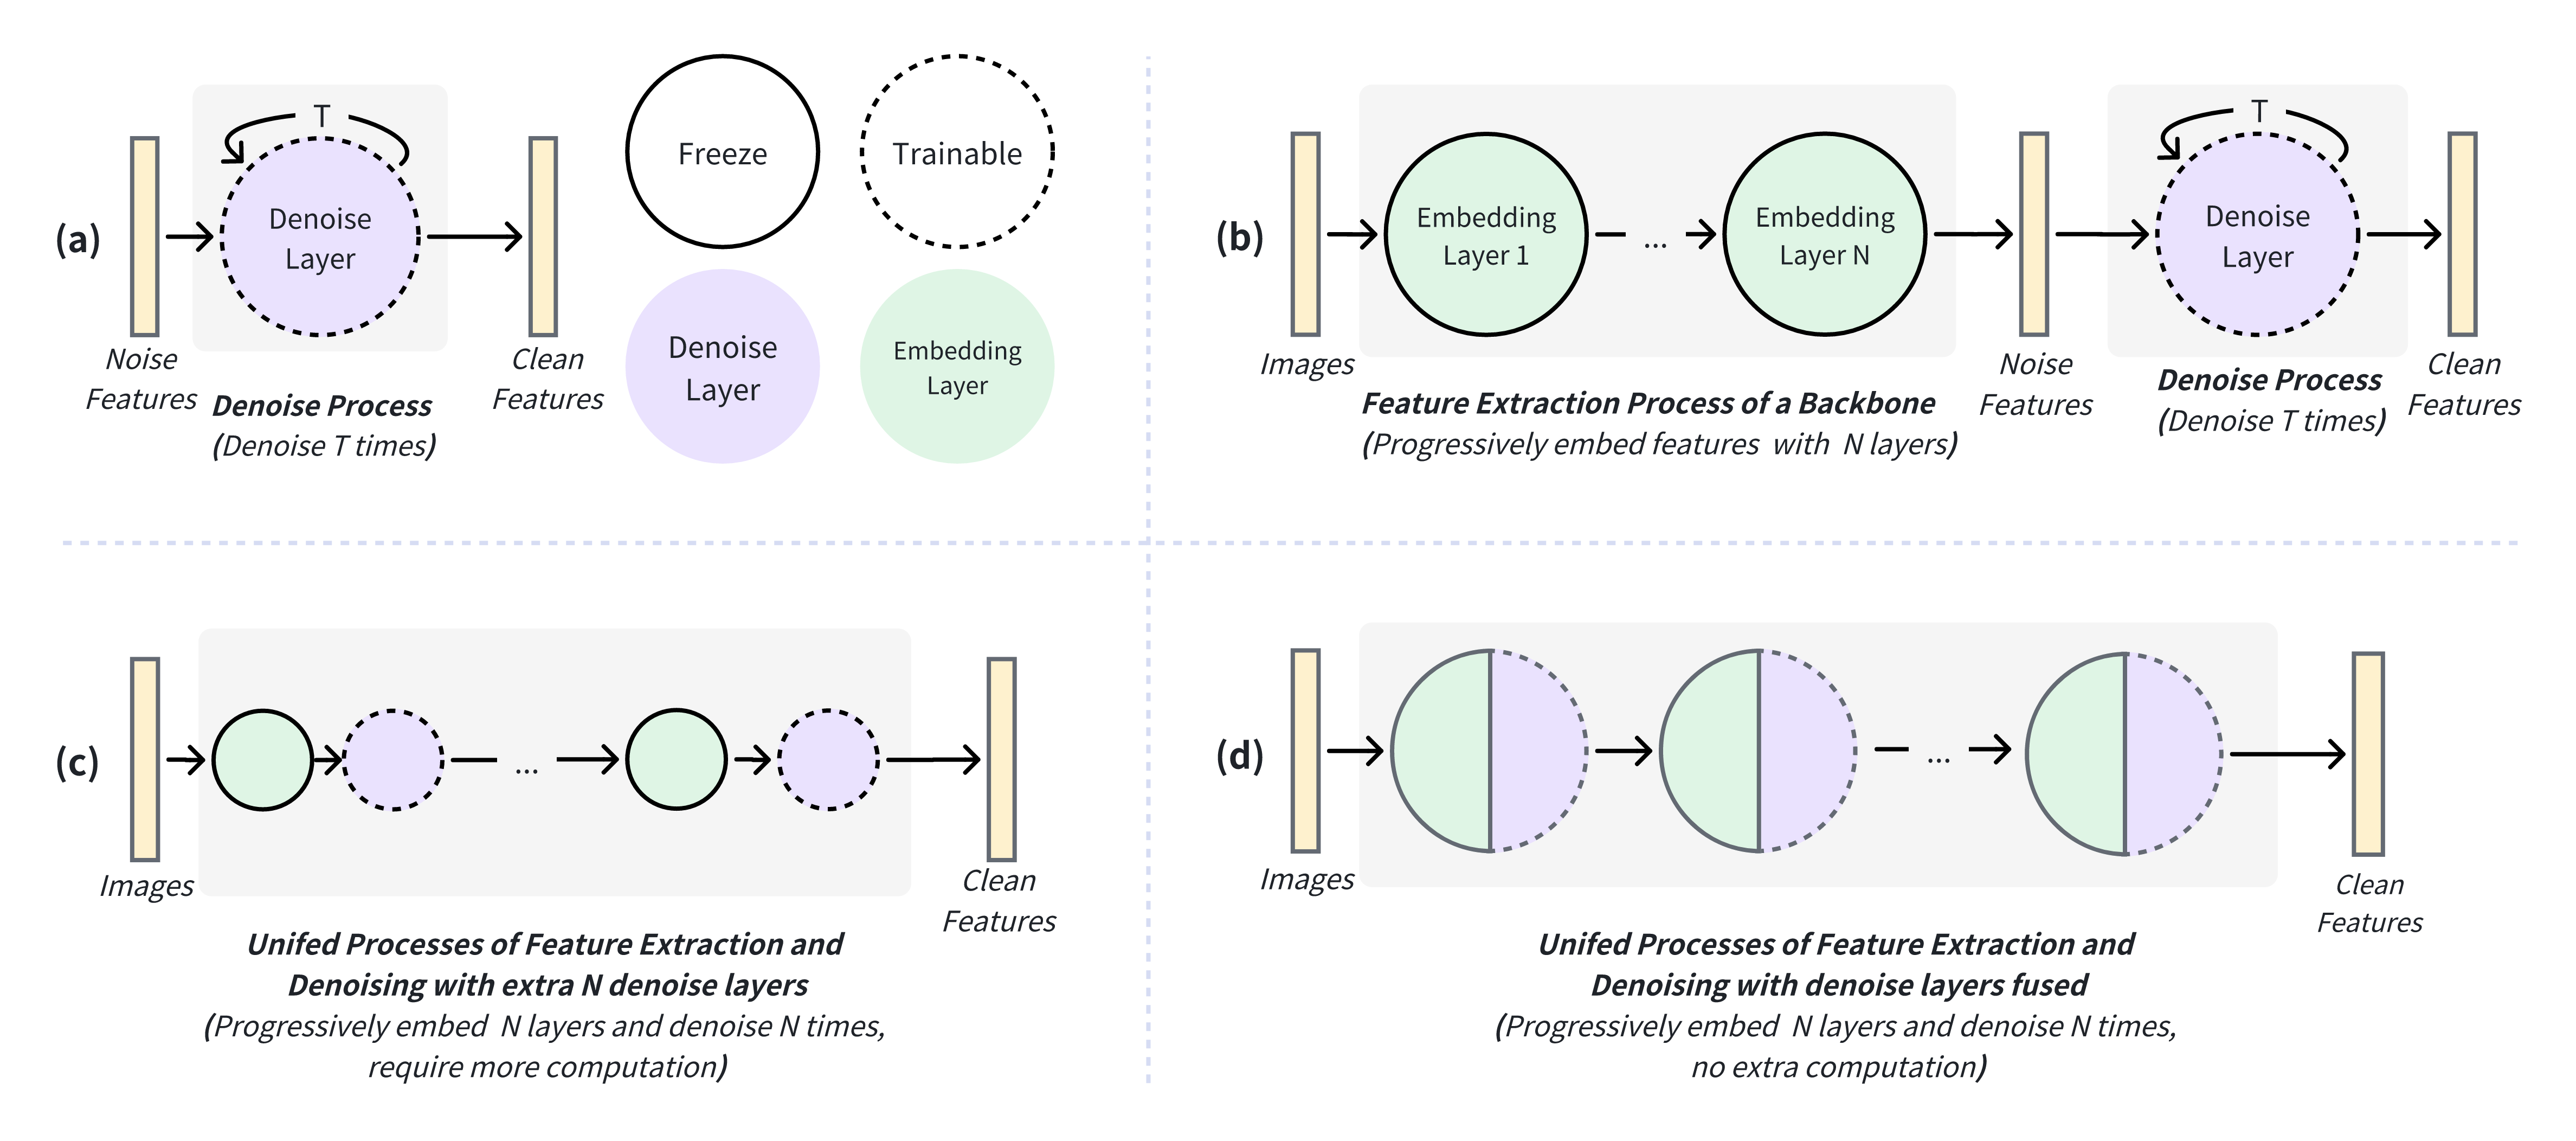
\includegraphics[width=\textwidth]{picture/intro5.png}
\caption{Illustration of our idea.
(a) A typical denoising model for generative tasks recursively applies a denoising layer.
(b) A naive extension to discriminative models applies a recursive denoising layer on backbone features, causing extra inference latency.
(c,d) Our \textit{DenoiseRep\textsuperscript{++}} unifies feature extraction and denoising in a backbone pipeline, then merges denoising parameters into embedding layers, making features more discriminative without extra latency.}
\label{pic:intro}
\end{figure*}

While these diffusion-based discriminative approaches have shown potential, they are typically tailored to specific applications and rely on particular data structures—for example, DiffusionDet~\cite{chen2023diffusiondet} operates on noisy bounding boxes, and DiffSeg~\cite{tian2023diffuse} on noise-initialized segmentations.
In this study, we explore a broader and more general question: how denoising models can facilitate representation learning, i.e., \textit{“learning representations (or features) of data that make it easier to extract useful information for building classifiers or other predictors”}~\cite{6472238}, thereby benefiting discriminative frameworks.
We employ person re-identification (ReID)~\cite{ye2021deep, bedagkar2014survey} as a benchmark, a task that aims to match pedestrian images across non-overlapping cameras and requires highly identity-discriminative features despite variations in pose, illumination, and occlusion.

A straightforward solution is to directly apply a denoising operation to the final-layer features of a backbone network~\cite{krizhevsky2012imagenet,dosovitskiy2020image}, as shown in Fig.~\ref{pic:intro}(b).
This may enhance feature discrimination but introduces significant computational overhead, since each denoising layer must sequentially process the output of the previous layer in a recursive fashion.
Considering that modern backbones inherently consist of cascaded embedding layers (e.g., convolutional or multi-head attention layers), we propose a novel interpretation: treating each embedding layer as an individual denoising layer.
As illustrated in Fig.~\ref{pic:intro}(c), this perspective allows the network to perform feature extraction and denoising in parallel across hierarchical layers, effectively transforming the backbone into a chain of progressive denoising operations.

However, implementing this idea is non-trivial because denoising layers typically require input and output features to reside in the same latent space, whereas conventional backbones (e.g., ResNet~\cite{krizhevsky2012imagenet} or ViT~\cite{dosovitskiy2020image}) gradually map features from low-level to high-level abstractions. This difference in feature spaces poses a major compatibility challenge.

To overcome these difficulties and effectively integrate denoising into discriminative pipelines, we propose the Enhanced Denoising Model for Representation Learning (\textit{DenoiseRep\textsuperscript{++}}), which consists of the following stages:
%
First, a pre-trained backbone network is utilized and kept frozen during subsequent training. This step leverages existing models freely available in the community and preserves their semantic feature extraction ability. Given an image input, the backbone provides a sequence of intermediate feature representations.
%
Second, denoising layers are trained on these extracted features. Their parameters are initialized independently and not shared across layers. The training process follows the DDPM~\cite{ho2020denoising} paradigm, except that DDPM employs a dynamic time step $t \in [1, T]$, while our denoising layers correspond to fixed indices $n \in [1, N]$, where $N$ denotes the number of backbone layers (see Fig.~\ref{pic:intro}(c)).
%
Finally, to mitigate the inference latency introduced by these $N$ denoising layers, we design a feature extraction–denoising fusion mechanism.
As shown in Fig.~\ref{pic:intro}(d), this method merges denoising parameters into the existing embedding layers, enabling unified feature extraction and denoising without any extra computational burden.
We further \textit{theoretically demonstrate} that the fused and unfused formulations are mathematically equivalent (see Eq.~(\ref{eq:One-step denoising (combined)})).


Building upon the \textit{DenoiseRep} framework, we introduce two synergistic extensions to resolve the inherent trade-off between denoising capacity and inference efficiency.
First, since the denoising module is designed to be lightweight for
seamless parameter fusion, this compact architecture limits its ability
to model complex, high-dimensional noise distributions, leading to
potential estimation bias. To address this, we employ a Teacher-Student Distillation paradigm. By leveraging a high-capacity teacher network to guide the lightweight student, we provide a more robust supervision signal that captures the uncertainty of noise patterns. This effectively calibrates the denoising direction, compensating for the student's limited parameter scale.
Second, single-step denoising often suffers from discretization errors when approximating the underlying data manifold. To mitigate this without increasing inference latency, we introduce Multi-step Denoising Fusion. This mechanism mathematically collapses a multi-round iterative process into a single linear operation. It functions as a trajectory optimization strategy, simulating a progressive refinement path that aligns features more tightly with their semantic centers.
Together, these enhancements enable \textit{DenoiseRep\textsuperscript{++}} to achieve superior feature discriminability—quantitatively evidenced by minimized intra-class variance and maximized inter-class separability—while strictly maintaining the computation-free inference property.



Our main contributions are summarized as follows:

(1) We propose a Enhanced Denoising Model for Representation Learning (\textit{DenoiseRep\textsuperscript{++}}), which integrates the generative denoising process into discriminative frameworks by interpreting $N$ cascaded embedding layers of a backbone as $T$ recursive denoising steps. This unification allows simultaneous feature extraction and denoising, leading to more discriminative representations.

(2) The proposed \textit{DenoiseRep\textsuperscript{++}} introduces a parameter fusion strategy that merges denoising and embedding layers, and \textit{theoretically proves} their equivalence, resulting in a computation-efficient framework with no additional inference latency.


(3) We introduce a high-capacity teacher--student distillation framework that employs a more expressive teacher network to guide the pre-noising module. This improves the accuracy of noise-distribution prediction and enhances the representational capacity of the denoising backbone without increasing inference cost.

(4) We introduce two denoising enhancement strategies, namely multi-round single-layer denoising and multi-step denoising fusion, which compress multi-step denoising trajectories into fewer effective steps. These methods enhance denoising performance and feature separability without increasing computational cost.


(5) Extensive experiments on four ReID datasets demonstrate that \textit{DenoiseRep\textsuperscript{++}} improves feature discrimination in a label-free manner and achieves even greater gains under supervised or augmented training settings.
Moreover, we extend our approach to large-scale (ImageNet), fine-grained (CUB200, Oxford-Pet, Flowers) classification, object detection (COCO), and image segmentation (ADE20K) tasks, confirming its robustness and scalability.

\section{Related Work}

\label{sec:formatting}

% \subsection{Generative Models}
\textbf{Generative models} aim to learn the underlying distribution of data before estimating class probabilities.
They capture the process by which data are generated through modeling the probability distribution of the inputs, thereby enabling the creation of new synthetic samples.
Typically, a generative model estimates the conditional likelihood of each class $P(x|y = k)$ along with the prior class probability $P(y = k)$ from training data, and then computes the marginal distribution $P(x)$ via the law of total probability.
This formulation allows the model to approximate the probability distribution for each category of data.
%
As a result, generative models can synthesize new data by sampling from the learned distribution.

Classic examples include Generative Adversarial Networks (GANs)~\cite{goodfellow2014generative,mirza2014conditional,karras2019style} and Variational Autoencoders (VAEs)~\cite{kingma2013auto,van2017neural,zhao2017learning,xu2022socialvae}, both of which generate realistic data by learning latent representations that capture the structure of the underlying distribution. These approaches have demonstrated outstanding performance in modeling data generation processes.
Recently, research attention has shifted toward \textbf{diffusion models} for generative tasks.
The diffusion framework was initially proposed by~\cite{sohl2015deep} to iteratively remove Gaussian noise from training images, and it was later popularized by the Denoising Diffusion Probabilistic Model (DDPM)~\cite{ho2020denoising}, which established diffusion as a mainstream approach to image synthesis.
Beyond their strong generative capacity, diffusion models also possess intrinsic denoising ability — through iterative noise estimation and removal, they can effectively restore the original data distribution from noisy observations.

% \subsection{Discrminative Models}
\textbf{Discriminative models}, in contrast, focus on learning the conditional probability distribution $P(y|x)$, where $x$ denotes input data and $y$ represents task-specific outputs or labels.
For instance, classification models~\cite{agarap2017architecture,albawi2017understanding,deng2012mnist} map inputs to discrete category labels; retrieval models~\cite{lin2015deep,weyand2020google} learn feature spaces in which semantically similar samples lie close together; and detection models~\cite{ren2015faster,law2018cornernet} localize and classify objects by predicting spatial positions and bounding boxes.

A prominent example of a discriminative task is \textbf{Person Re-Identification (ReID)}, which seeks to identify the same individual across non-overlapping camera views.
Due to challenges such as pose variation, illumination change, and occlusion, ReID requires highly discriminative features.
Accordingly, we employ ReID as our primary benchmark and use other tasks as auxiliary validation.
Existing ReID techniques can generally be categorized into (1) hand-crafted descriptors~\cite{liao2015person,ma2014covariance,yang2014salient} combined with metric learning~\cite{koestinger2012large,liao2015efficient,zheng2013reidentification}, and (2) deep learning–based approaches~\cite{wang2020high,wang2019color,wang2023self,ni2023part,fu2021unsupervised,cho2022part}.
Modern ReID systems predominantly adopt convolutional neural networks (CNNs)~\cite{lecun1998gradient} to model complex spatial relationships and hierarchical visual representations.
Furthermore, attention mechanisms~\cite{vaswani2017attention,dosovitskiy2020image}, spatio-temporal reasoning~\cite{li2020dyngcn,li2022autost}, and domain adaptation methods~\cite{chen2018domain} have further enhanced their robustness and generalization to real-world deployment scenarios.

\textbf{Efficient Diffusion Sampling.} One of the central challenges of diffusion models is their high computational cost during inference, as conventional denoising procedures typically require hundreds or even thousands of iterative steps. To mitigate this inefficiency, a series of accelerated sampling techniques have been proposed in recent years.

DDPM~\cite{ho2020denoising} established the fundamental iterative denoising framework, which achieves high-quality sample generation but suffers from long inference times.
To improve efficiency, the Denoising Diffusion Implicit Model (DDIM)~\cite{song2020denoising} introduced a deterministic, non-Markovian reformulation that maintains visual quality with significantly fewer sampling steps.
Building upon this idea, Progressive Distillation ~\cite{salimans2022progressive} iteratively halves the required sampling steps by training a student model to match the output of a teacher that performs two consecutive denoising steps. This effectively compresses a long diffusion trajectory into fewer steps without significant loss of quality.
More recently, DPM-Solver~\cite{lu2022dpm} formulated the diffusion process as an ordinary differential equation (ODE) and employed high-order numerical solvers to approximate denoising trajectories efficiently, reducing sampling steps to as few as 10–20 without sacrificing fidelity.

These advancements collectively reflect the growing focus on balancing denoising precision and computational efficiency in diffusion models.
Our work draws inspiration from such accelerated sampling strategies—particularly distillation-based methods—in designing the step-wise distillation and multi-round denoising mechanisms that enhance \textit{DenoiseRep\textsuperscript{++}} under limited computational budgets.

\section{\textit{DenoiseRep\textsuperscript{++}}: Enhanced Denoising Model for Representation Learning}
{\color{black}
% \subsection{Review Representation Learning of Person Re-Identification}
\subsection{Review Representation Learning}

Representation learning serves as a cornerstone for discriminative tasks and is formally defined as \textit{"the process of learning representations (or features) of data that facilitate the extraction of meaningful information for constructing classifiers or other predictive models"}~\cite{6472238}.
A typical discriminative framework comprises a vision backbone responsible for extracting task-relevant features (\textit{e.g.}, ResNet~\cite{he2016deep}, ViT~\cite{dosovitskiy2020image}) and a task-specific head that operates upon these features (\textit{e.g.}, MLP~\cite{krizhevsky2012imagenet} for classification, RCNN~\cite{ren2015faster} for detection, or FCN~\cite{long2015fully} for segmentation).
It is thus apparent that the vision backbone plays a fundamental role in representation learning, as it determines the quality and discriminability of the extracted features.
%
In this work, we propose a novel framework, termed the Enhanced Denoising Model for Representation Learning (\textit{DenoiseRep\textsuperscript{++}}), which unifies feature extraction and denoising within a single backbone architecture.
By integrating these two processes, \textit{DenoiseRep\textsuperscript{++}} aims to strengthen the discriminative capacity of learned representations while maintaining computational efficiency.



% \subsection{Feature Extraction and Feature Denoising Unified Framework}
\subsection{Joint Feature Extraction and Feature Denoising}


We refer to the diffusion modeling approach to denoise the noisy features through T-steps to obtain clean features. At the beginning, we use the features output from the backbone network as data samples for diffusion training, and get the noisy samples by continuously adding noise and learning through the network in order to simulate the data distribution of its features. 
%
\begin{align}
q(\mathbf{x}_{1:T} | \mathbf{x}_0) &\coloneqq \prod_{t=1}^T q(\mathbf{x}_t | \mathbf{x}_{t-1}) \qquad \\
q(\mathbf{x}_t|\mathbf{x}_{t-1}) &\coloneqq \mathcal{N}(\mathbf{x}_t; \sqrt{1-\beta_t}\mathbf{x}_{t-1}, \beta_t \mathbf{I}) \label{eq:forwardprocess}
\end{align}
where $X_0$ represents the feature vector output by the backbone, $t$ represents the diffusion step size, $\beta_t$ is a set of pre-set parameters, and $X_t$ represents the noise sample obtained through diffusion process.

%
In the inference stage, as shown in Fig.~\ref{pic:intro}(b), we perform T-step denoising on the output features, to obtain cleaner features and improve the expressiveness of the features.
\begin{align}
  p_\theta(\mathbf{x}_{0:T}) &\coloneqq p(\mathbf{x}_T)\prod_{t=1}^T p_\theta(\mathbf{x}_{t-1}|\mathbf{x}_t) \\ 
  p_\theta(\mathbf{x}_{t-1}|\mathbf{x}_t) &\coloneqq \mathcal{N}(\mathbf{x}_{t-1}; \mu_\theta(\mathbf{x}_t, t), \Sigma_\theta(\mathbf{x}_t, t))
\end{align}
where $X_t$ represents the feature vector output by the backbone in the inference stage. $T$ is the denoising step size, representing the magnitude of the noise. We adjust $t$ appropriately based on different datasets and backbones to obtain the optimal denoising amplitude.
% In ViT-base and ViT-small backbone, $t$ is set to 10 and 15, respectively.
According to $p_\theta(\mathbf{x}_{t-1}|\mathbf{x}_t)$ denoise it step by step, and finally obtains $X_0$, which represents the clean feature after denoising.



\label{sec:methods ED Module}


% \subsection{Denoise module}


% \vspace{-5em}
\begin{figure*}[t]
\vspace{-2em}
    \centering
    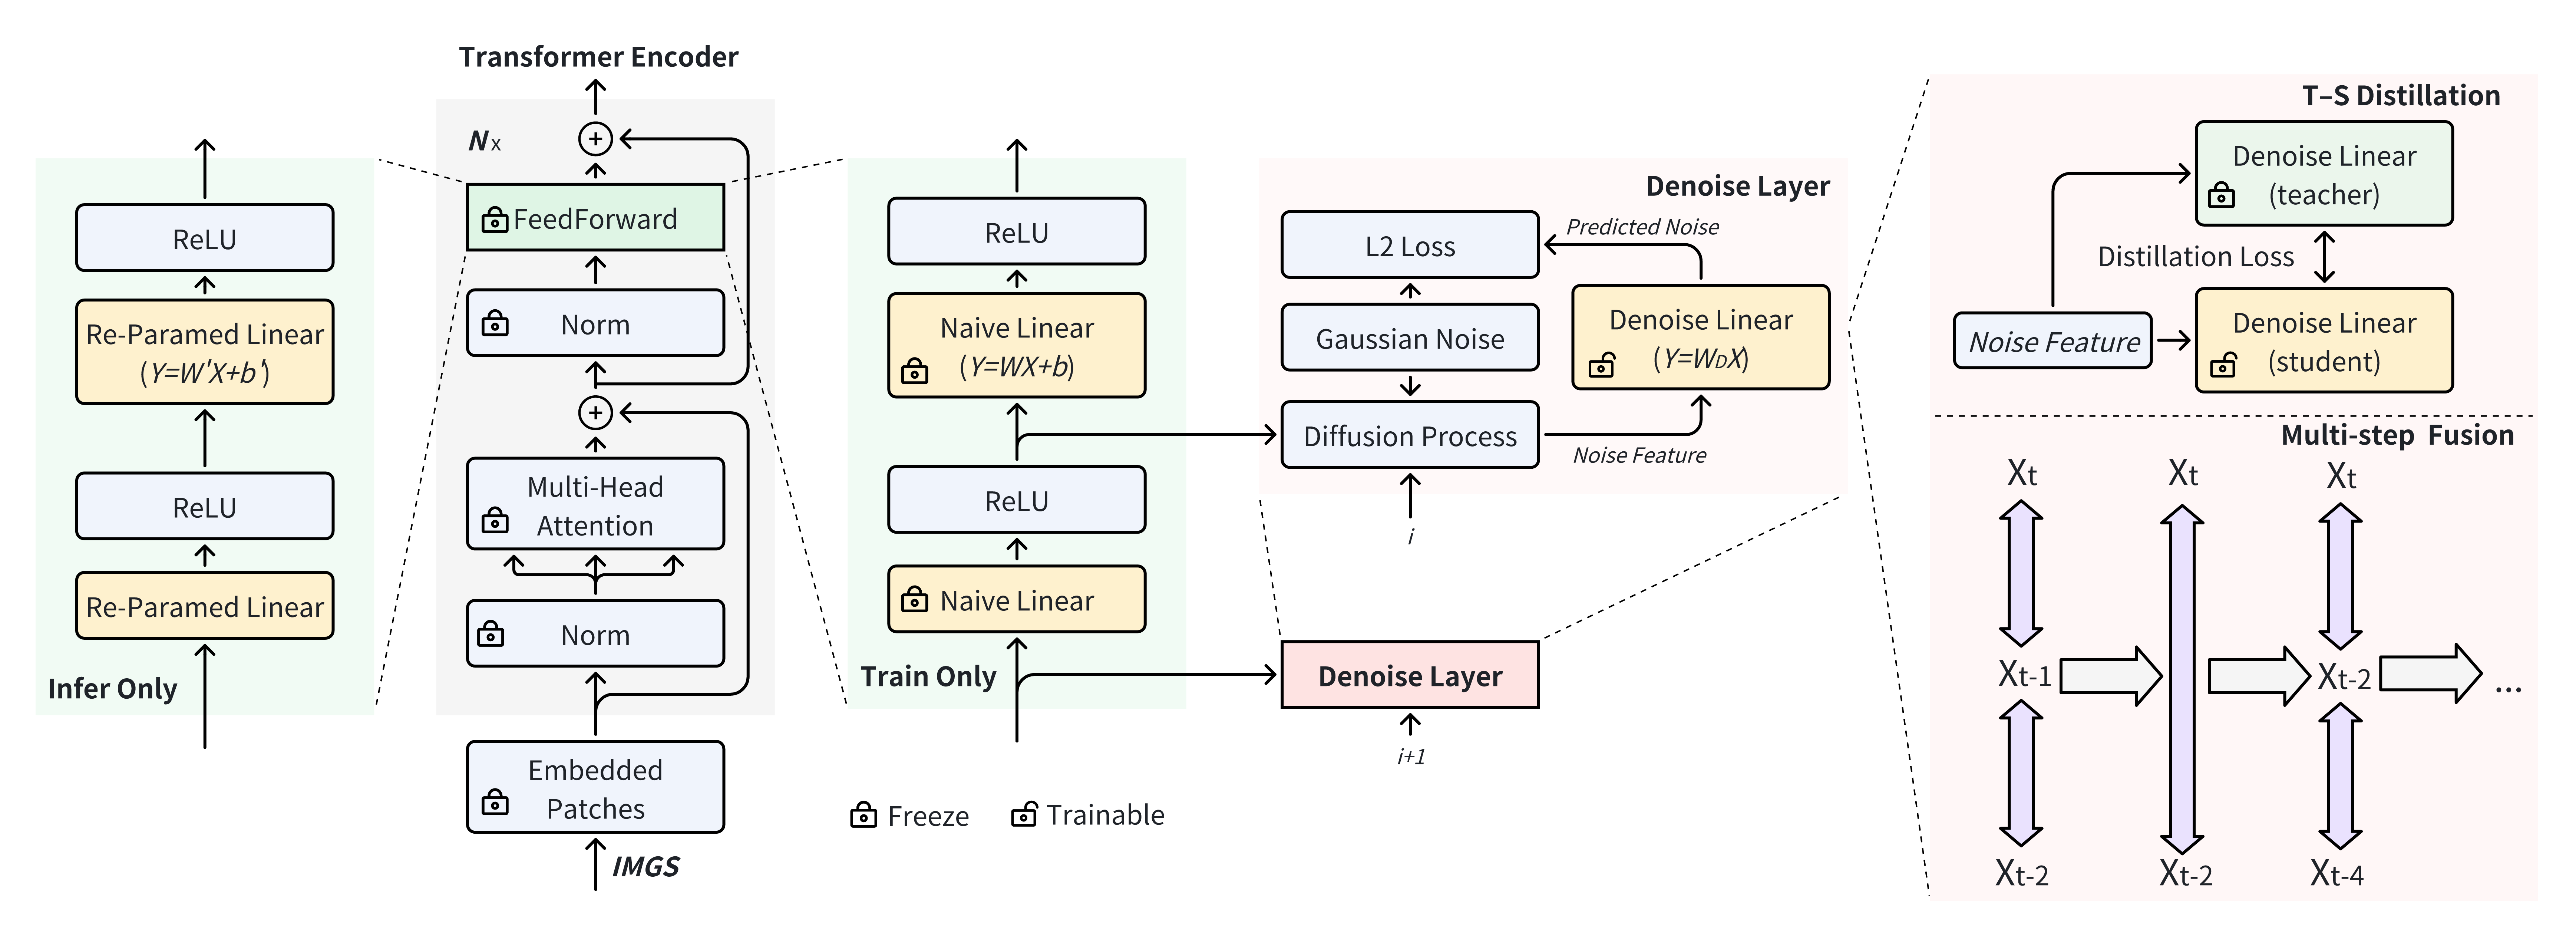
\includegraphics[width=\textwidth]{picture/train2.png}
    \caption{Pipeline of the proposed \textit{DenoiseRep\textsuperscript{++}}. 
    The Vision Transformer (ViT) consists of $N$ cascaded transformer encoder layers. 
    During training (right, ``Train Only''), the backbone parameters are frozen and only the additional denoising layers are optimized. This phase also incorporates T-S (Teacher-Student) Distillation and supports a Multi-Step Fusion process for iterative refinement. During inference (left, ``Infer Only''), the parameters of denoising layers are merged into the corresponding encoder layers, introducing no extra inference latency. 
    Definitions of $W$, $b$, $W_{D}$, $W'$, $i$, and $b'$ are provided in Algorithm~\ref{alg:Inference}.}
    \label{pic:train}
\end{figure*}

% \subsection{Feature Extraction and Feature Denoising Fusion Algorithm}
\subsection{Fuse Feature Extraction and Feature Denoising}

\label{sec:method RD Plugin}
As described in Section \ref{sec:methods ED Module}, the proposed method above could effectively improve the discriminability of features. Still, extra inference latency is introduced caused by recursive calling of the denoising layers.
%
To solve the problem, we propose to fuse parameters of feature denoising layers into parameters of existing embedding layers of the backbone. The core idea is to expand the linear layer each transformer encoder block into two branches, one for its original embedding layer and the other for extra denoising layer. As shown in Fig.~\ref{pic:train}, during the training phase, we freeze the original embedding layers and only train the denoising layers. The training method is consistent with section \ref{sec:methods ED Module}, and the features are diffused and fed into the denoising layers. Please refer to Algorithm \ref{alg:Training} for more details. In the inference stage, we fuse the pre-trained parameters of embedding and denoising layers, merging the two branches into a single branch without additional inference time. 
%
Please note that, here we take the transformer architecture as an example, but \textit{DenoiseRep\textsuperscript{++}} is suitable for CNN architecture. We demonstrate its scalibity on CNN in experiments.
%
The derivation of parameter merging is as follows:
\begin{equation}
% %\vspace{-0.1cm}
X_{t-1} =\frac{1}{\sqrt{a_t} } (X_t - \frac{1-a_t}{\sqrt{1 - \bar{a_t} } } D_\theta(X_t, t))+\sigma_tz \label{eq:one-step denoising}
% %\vspace{-0.8cm}
\end{equation}
where $a_t = 1- \beta_t$, $D_\theta$ are the parameters of the prediction noise network.
\begin{equation}
\begin{aligned}
     Y &= WX + b \\
     \frac{1}{\sqrt{a_t} }X_t - X_{t-1} &= \frac{1-a_t}{\sqrt{a_t}\sqrt{1-\bar{a_t} }  }D_\theta X_t-\sigma_tz   \\
     \frac{1}{\sqrt{a_t} }Y_t - Y_{t-1} &= \frac{1-a_t}{\sqrt{a_t}\sqrt{1-\bar{a_t} }  }D_\theta Y_t-\sigma_tz 
\end{aligned}
\label{eq:One-step denoising (transform)}
\end{equation}
We make a simple transformation of Eq. (\ref{eq:one-step denoising}) and multiply both sides simultaneously by $W$.
The simplified equation can be obtained by bringing $Y_t$ in terms of $WX_t + b$:
\begin{equation}
\begin{aligned}
     Y_{t-1} = [W - C_1(t) &WW_D]X_t+WC_2(t)C_3 + b  \\
     C_1(t)  &= \frac{1-a_t}{\sqrt{a_t}\sqrt{1-\bar{a_t} }  }\\
     C_2(t) &= \frac{1-\bar{a_{t-1}}}{1-\bar{a_t}} \beta_t\\
     C_3  &= Z\sim N(0, I)
\end{aligned}
\label{eq:One-step denoising (combined)} 
\end{equation}
where $W_D$ denotes the parameters of $D_\theta(X_t, t)$, $X_t$ denotes the input of this linear layer, $Y_t$ denotes the output of this linear layer, and $Y_{t-1}$ denotes the result after denoising in one step of $Y_t$. Due to the cascading relationship of blocks, as detailed in Algorithm. \ref{alg:Inference}, different $t$ values are set according to the order between levels, and the one-step denoising of one layer is combined to achieve the denoising process of $Y_t \rightarrow Y_0$, ensuring the continuity of denoising and ultimately obtaining clean features. We split the original single branch into a dual branch structure. During the training phase, the backbone maintains its original parameters and needs to train the denoising module parameters. In the inference stage, as shown on the left side of Fig.~\ref{pic:train}, we use the method of reparameterization, to replace the original $W$ parameter with $W'$, where $W' = [W - C_1(t) WW_D]$ in Eq. (\ref{eq:One-step denoising (combined)}), which has the same number of parameters as $W$, thus achieving the combination of $FC$ operation and denoising without additional time cost. It is a \textbf{Computation-free} method.


In Eq. (\ref{eq:One-step denoising (combined)}), we achieve one-step denoising $Y_t \rightarrow Y_{t-1}$. If we need to increase the denoising amplitude, we can extend it to two-step or multi-step denoising. The following is the derivation formula for two-step denoising:
\begin{equation}
% %\vspace{-0.3cm}
     \frac{1}  {\sqrt{a_t} }Y_t - Y_{t-1} = C_1(t)D_\theta Y_t-\sigma_tz \label{eq:one-step denoising in Yt}
% %\vspace{-0.5cm}
\end{equation}
% %\vspace{-0.3cm}
\begin{equation}
     \frac{1}{\sqrt{a_{t-1}} }Y_{t-1} - Y_{t-2} = C_1(t-1)D_\theta Y_{t-1}-\sigma_{t-1}z \label{eq:one-step denoising in Yt-1}
\end{equation}
We can obtain this by eliminating $Y_{t-1}$ from Eq.(\ref{eq:one-step denoising in Yt}) and Eq.(\ref{eq:one-step denoising in Yt-1}) and replacing $Y_t$ with $WX_t+b$:
\begin{equation}
\begin{aligned}
    &\quad\quad\quad\quad Y_{t-2} = W''X_t + C'' \\[6pt]
    W'' &= \frac{1}{\sqrt{(a_t-1)}}\Bigg\{ 
        \frac{W}{\sqrt{a_t}} 
        - \big[C_1(t) + C_1(t-1)\big] W W_D  \\
        &\quad + \sqrt{a_t}\, C_1(t-1) C_1(t) W W_D W_D \Bigg\}, \\[6pt]
    C'' &= \frac{1}{\sqrt{(a_t-1)}} \Big[ 
        W C_2(t) + \sqrt{a_t}\, W C_2(t-1)  \\
        &\quad - \sqrt{a_t}\, C_1(t-1) C_2(t) W W_D \Big] Z + b .
\end{aligned}
\label{eq:two_step_denoising}
\end{equation}
Note that a single module completes two steps of denoising. To ensure the continuity of denoising, the $t$ value should be sequentially reduced by 2.

Our proposed \textit{DenoiseRep\textsuperscript{++}} is based on feature-level denoising and can be migrated to various downstream tasks. It denoises the features on each layer for better removal of noise at each stage, as the noise in the inference stage comes from multiple sources, which could be noise in the input image or noise generated while passing through the network. Denoising each layer avoids noise accumulation and gives better quality output. And according to the noise challenges brought by data in different scenarios, the denoising intensity can be adjusted by controlling $t$, $\beta_t$, and the number of denoising times, which has good generalization ability.

\begin{algorithm}[t]
	\renewcommand{\algorithmicrequire}{\textbf{Input:}}
	\renewcommand{\algorithmicensure}{\textbf{Output:}}
	\caption{Training}
	\label{alg:Training}
	\begin{algorithmic}[1]
		\Require The number of feature layers in the backbone N, features extracted from each layer $\{F_i\}_{i=1}^{N} $, the denoising module that needs to be trained $\{D_i(\cdot )\}_{i=1}^{N}$.
            \Repeat
		\For {each $i \in [N,1]$}
		\State $t = i$: Specify the diffusion step t for the current layer based on the order of layers.
		\State $\epsilon \sim N(0,I)$: Randomly sample a Gaussian noise.
            \State $X_t = \sqrt{\bar{a_t} }F_i+\sqrt{1-\bar{a_t} } \epsilon$:  Forward diffusion process in Eq.(\ref{eq:forwardprocess}).
		\State Take gradient descent step on 
                    $\nabla _\theta \left \| \epsilon-D_i(X_t,t )  \right \|^{2} $
            
            \EndFor
		\Until{converged}
	\end{algorithmic}  
\end{algorithm}

\begin{algorithm}
	\renewcommand{\algorithmicrequire}{\textbf{Input:}}
	\renewcommand{\algorithmicensure}{\textbf{Output:}}
	\caption{Inference}
	\label{alg:Inference}
	\begin{algorithmic}[1]
		\Require The number of feature layers in the backbone N, features extracted from each layer $\{F_i\}_{i=1}^{N} $, trained denoising module parameters $\{W_{D_i}\}_{i=1}^{N}$ in Algorithm(\ref{alg:Training}), after obtaining the initial feature $F^{N}$ through patch\_embed, it is necessary to remove N-step noise from it, the pre-trained parameters $\{W_i\}_{i=1}^{N} $ and $\{b_i\}_{i=1}^{N} $ for the backbone.
		\Ensure Feature $F^{0}$ after denoising.
		\For {each $i \in [N,1]$}
		\State $t = i$: Set the denoising amplitude based on the depth of the current layer.
            \State $W' = [W_i - C_1(t) W_iW_{D_i}]$, 
            $b' = W_iC_2(t)C_3 + b_i$: Parameter fusion according to Eq.(\ref{eq:One-step denoising (combined)}).
            \State $F^{t-1} = W'F^{t} + b'$: Fuse feature extraction and feature denoising.
	\EndFor
		\State \textbf{return} $F^{0}$
	\end{algorithmic}  
% %\vspace{-0.1cm}
\end{algorithm}




\subsection{Teacher--Student Distillation for Denoising Module}
\label{sec:method_distill}

As discussed in previous sections, the denoising module is designed to be lightweight in order to support parameter fusion with backbone layers at inference time. However, such a compact architecture inevitably limits its capacity to accurately predict noise distributions, leading to sub-optimal denoising effectiveness. As illustrated in Fig.~\ref{fig:teacher_student_distill}, we address this limitation by adopting a teacher--student distillation framework during training.


\begin{figure}[t]
    \centering
    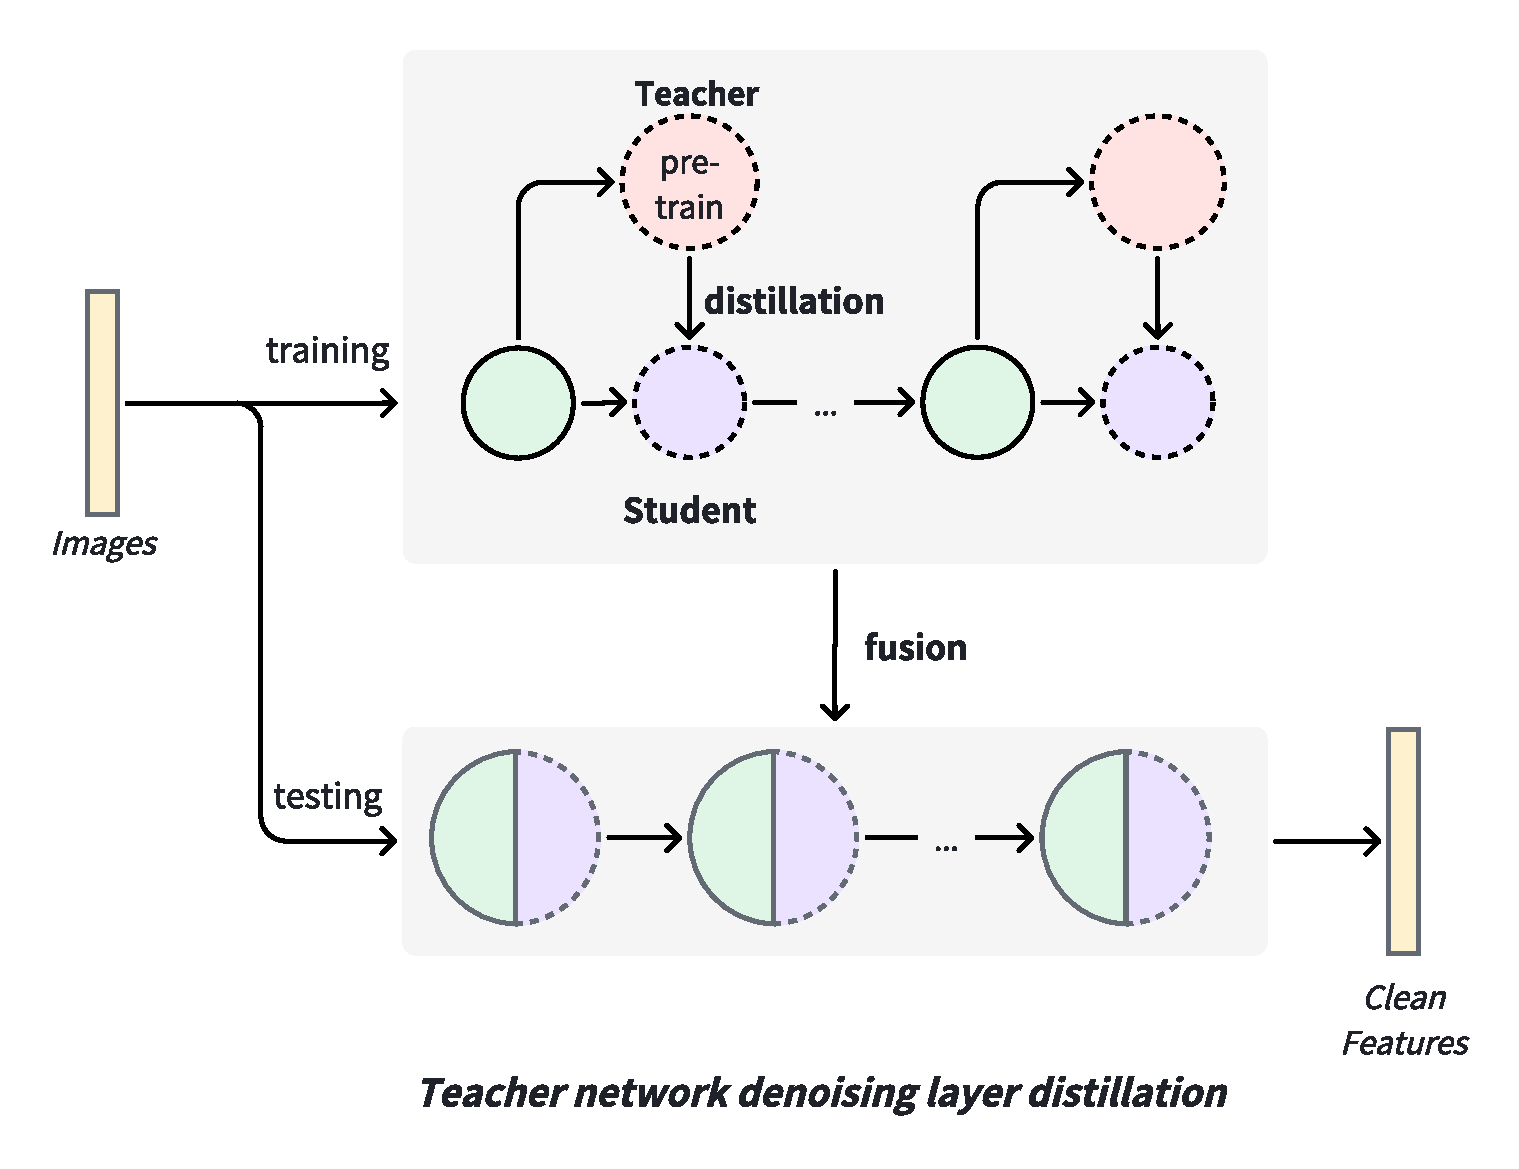
\includegraphics[width=0.95\columnwidth]{picture/denoising_layer_distillation.pdf}
    \caption{Illustration of the teacher--student denoising layer distillation framework. 
    During training, a strong teacher network supervises the student denoising module through feature-level distillation. 
    The trained student is then fused with the backbone for computation-free inference, 
    producing clean and discriminative features.}
    \label{fig:teacher_student_distill}
\end{figure}

In particular, we construct a more expressive teacher network that serves as a strong denoiser. Given the same noisy feature $X_t$ at diffusion step $t$, the teacher network outputs a noise prediction $\hat{\epsilon}_T(X_t, t)$, while the student network outputs $\hat{\epsilon}_S(X_t, t)$. We treat the teacher’s prediction as a soft label and train the student to regress toward it using an L2 objective:  

\begin{equation}
\mathcal{L}_{distill} = \left\| \hat{\epsilon}_S(X_t, t) - \hat{\epsilon}_T(X_t, t) \right\|_2^2 .
\label{eq:distill}
\end{equation}

The final training objective is a weighted sum of the original denoising loss and the distillation loss:  
\begin{equation}
\mathcal{L}_{total} = \lambda_p \mathcal{L}_{denoise} + \lambda_d \mathcal{L}_{distill},
\label{eq:total_distill}
\end{equation}
where $\lambda_p$ and $\lambda_d$ are balancing coefficients.  

\begin{algorithm}[t]
    \renewcommand{\algorithmicrequire}{\textbf{Input:}}
    \renewcommand{\algorithmicensure}{\textbf{Output:}}
    \caption{Teacher--Student Distillation Training}
    \label{alg:distill}
    \begin{algorithmic}[1]
        \Require Features $\{F_i\}_{i=1}^N$, student denoiser $\{D^S_i(\cdot)\}$, teacher denoiser $\{D^T_i(\cdot)\}$.
        \Repeat
            \For {each $i \in [N,1]$}
                \State $t = i$; sample noise $\epsilon \sim N(0, I)$
                \State $X_t = \sqrt{\bar{a_t}}F_i + \sqrt{1-\bar{a_t}} \epsilon$
                \State Teacher prediction: $\hat{\epsilon}_T = D^T_i(X_t, t)$
                \State Student prediction: $\hat{\epsilon}_S = D^S_i(X_t, t)$
                \State Update student by minimizing $\mathcal{L}_{distill}$ in Eq.~(\ref{eq:distill})
            \EndFor
        \Until{converged}
    \end{algorithmic}
\end{algorithm}

By leveraging the teacher’s stronger representational capacity, the student denoising module is able to more accurately approximate noise distributions. Importantly, this additional cost is only incurred during training, while the inference procedure remains efficient and computation-free.  




\subsection{Enhanced Denoising under Limited Layers}
\label{sec:method_multi}

Although \textit{DenoiseRep\textsuperscript{++}} fuses denoising with feature extraction, its denoising strength is inherently bounded by the number of available layers. To address this challenge, we introduce two complementary techniques: multi-round single-layer denoising and step-wise distillation.  

\textbf{Multi-round single-layer denoising.}  
Instead of relying solely on the depth of the network, we allow a single denoising layer to be applied iteratively across multiple rounds. This simulates a deeper denoising trajectory without introducing additional parameters. The basic one-step denoising update is defined as:  
\begin{equation}
X_{t-1} = \frac{1}{\sqrt{a_t}} \Big( X_t - \frac{1-a_t}{\sqrt{1-\bar{a_t}}}\,\epsilon_\theta(X_t,t) \Big) + \delta_t z,
\label{eq:multi_basic}
\end{equation}
where $\epsilon_\theta(X_t,t)$ is the noise predicted by the denoiser, and $\delta_t z$ is the Gaussian perturbation.  

Assuming a linear layer $G_\theta(X_t,t) = W X_t + b$, Eq.~(\ref{eq:multi_basic}) can be rewritten as:  
\begin{equation}
X_{t-1} = \sqrt{a_t}\Big(I - \tfrac{1-a_t}{\sqrt{1-\bar{a_t}}} W \Big)X_t - \tfrac{1-a_t}{\sqrt{1-\bar{a_t}}} b + \delta_t z.
\label{eq:multi_affine}
\end{equation}

Defining $A_t = \sqrt{a_t}(I - \tfrac{1-a_t}{\sqrt{1-\bar{a_t}}}W)$ and $C_t = -\tfrac{1-a_t}{\sqrt{1-\bar{a_t}}}b$, the recursion simplifies to:  
\begin{equation}
X_{t-1} = A_t X_t + C_t + \delta_t z.
\label{eq:multi_recursive}
\end{equation}

By applying Eq.~(\ref{eq:multi_recursive}) recursively for $k$ steps, we obtain the multi-round denoising result:  
\begin{equation}
\begin{aligned}
X_{t-k} &= A_{t-1} A_{t-2} \cdots A_{t-k} X_t  \\
&\quad + \sum_{j=0}^{k-1} \Big( \prod_{i=j+1}^{k} A_{t-i} \Big) C_{t-j}  \\
&\quad + \sum_{j=0}^{k-1} \Big( \prod_{i=j+1}^{k} A_{t-i} \Big) \delta_{t-j} z .
\end{aligned}
\label{eq:multi_kstep}
\end{equation}

Finally, the feature output after fusion with the linear layer is expressed as:  
\begin{equation}
Y_0 = W_L \big( A_t X_t + C_t + \delta_t z \big) + b_L ,
\label{eq:multi_output}
\end{equation}
which can be abstracted as a fusion operation
\begin{equation}
Y_0 = f_{\text{fusion}}(X_t, t, W_L, b_L, W, b).
\label{eq:fusion_func}
\end{equation}



\begin{algorithm}[t]
\caption{Multi-step Denoising Fusion}
\label{alg:multi_step_fusion}
\renewcommand{\algorithmicrequire}{\textbf{Input:}}
\renewcommand{\algorithmicensure}{\textbf{Output:}}
\begin{algorithmic}[1]

\Require Training samples $x$, diffusion step $t$, noise schedule $\{\beta_t\}$,
teacher denoiser $D_T$, student denoiser $D_S$
\Ensure Fused student model capable of multi-step denoising in one step

\State \textbf{Stage 1:} Teacher Training
\For{each minibatch $x$}
    \State Sample noise $\epsilon \sim \mathcal{N}(0,I)$
    \State Diffuse clean input: $z_t = \sqrt{\bar{a}_t}x + \sqrt{1-\bar{a}_t}\epsilon$
    \State Teacher predicts noise $\hat{\epsilon}_T = D_T(z_t, t)$
    \State Update teacher using loss $\mathcal{L}_\theta = \|\epsilon - \hat{\epsilon}_T\|_2^2$
\EndFor

\State \textbf{Stage 2:} Teacher Multi-Step Denoising (DDIM-style Skip Sampling)
\For{each training step}
    \State Teacher multi-step update $z_t \rightarrow z_{t-k} \rightarrow \hat{x}$,
    where $k \ge 2$ is the skip interval
\EndFor

\State \textbf{Stage 3:} Student One-Step Prediction
\For{each minibatch}
    \State Student predicts one-step result $\hat{x}_S = D_S(z_t, t)$
    \State Compute fusion loss
    $\mathcal{L}_{fusion} = w(\lambda_t)\|\hat{x} - \hat{x}_S\|_2^2$
    \State Update student parameters using $\mathcal{L}_{fusion}$
\EndFor

\State \textbf{Return} fully trained student model capable of approximating
multi-step denoising in a single step

\end{algorithmic}
\end{algorithm}


\textbf{Multi-step denoising fusion.}  
In addition to the recursive multi-round strategy, we further adopt a multi-step fusion scheme inspired by progressive distillation in diffusion models. The key idea is to replace multiple small denoising steps with a single larger step, while transferring the supervision from a pre-trained teacher network.  

The standard denoising training objective for the teacher is:
\begin{equation}
\mathcal{L}_{\theta} = \left\| \epsilon - \hat{\epsilon}_{\theta}(z_t, t) \right\|_2^2 ,
\label{eq:teacher_loss}
\end{equation}
where $\epsilon$ denotes the sampled Gaussian noise, $z_t$ is the noisy input at step $t$, and $\hat{\epsilon}_{\theta}$ is the teacher’s noise prediction.  

Once a strong teacher model is obtained, we employ a DDIM-style skip sampling rule, where the teacher predicts over two (or more) steps, and the student learns to approximate the same result in a single step. The corresponding distillation loss is:
\begin{equation}
\mathcal{L}_{\theta}^{\text{fusion}} = w(\lambda_t) \, \left\| \hat{x} - \hat{x}_{\theta}(z_t, t) \right\|_2^2 ,
\label{eq:fusion_loss}
\end{equation}
where $\hat{x}$ is the denoised output predicted by the teacher after multiple steps, $\hat{x}_{\theta}(z_t, t)$ is the student’s one-step prediction, and $w(\lambda_t)$ is a weighting function.  

This formulation enables the student to perform multi-step denoising in a single pass, effectively fusing multiple denoising operations into one. The distillation process progressively compresses longer trajectories into fewer steps, while maintaining denoising effectiveness.




\subsection{Unsupervised Learning Manner}
\label{sec:methods label-free}
Our proposed \textit{DenoiseRep\textsuperscript{++}} is label-free because its essence is a generative model that models data by learning its distribution. Thus the training loss contains only the $Loss_p$ of denoising layers:
\begin{equation}
% %\vspace{-0.1cm}
     % Loss_p = \left \|\epsilon  - D_\theta(X_t, t)  \right \| 
      Loss_{p} = \sum_{i = 1}^{N}\left |  \epsilon_{i} - D_{\theta _{i}}(X_{t_{i}}, t_{i})   \right |  
\end{equation}
where $\epsilon$ denotes the sampled noise, $N$ denotes the number of denoising layers, $X_t$ denotes the noise sample, $t$ denotes the diffusion step, and $D_\theta(X_t, t)$ denotes the noise predicted by the denoising layer.

However, it is worth noting that our method is complementary to label if the label is available. $Loss_{l}$ is the task-specific supervised loss with label, $\lambda$ is the trade-off parameter between two losses. The label-argumented learning is defined as: 

%
\begin{equation}
% %\vspace{-0.1cm}
     Loss = (1-\lambda)Loss_{l} + \lambda Loss_p
\end{equation}
Results in experiments Section~\ref{sec: Exp RD Plugin} shows the improvement from label.


\section{Experiments}


\begin{adjustwidth}{-1cm}{-1cm}
\begin{table*}[ht!]
\begin{center}
\caption{Experimental results on various discriminative tasks. }
\vspace{0.0cm}
\label{tab: performance on multiple image tasks.}
\begin{tabular}{lcccc|cc}
\hline \hline
\begin{tabular}[c]{@{}c@{}}Task\end{tabular} &
\begin{tabular}[c]{@{}c@{}}Model\end{tabular} &
\begin{tabular}[c]{@{}c@{}}Backbone\end{tabular} & 
\begin{tabular}[c]{@{}c@{}}Dataset\end{tabular} & 
\begin{tabular}[c]{@{}c@{}}Metric\end{tabular} & 
\begin{tabular}[c]{@{}c@{}}\textit{Baseline}\end{tabular} & 
\begin{tabular}[c]{@{}c@{}}\textit{\textbf{+DenoiseRep\textsuperscript{++}}}\end{tabular} 
\\
\hline
Classification & SwinT~\cite{liu2021swin}   & SwinV2-T & ImageNet-1k & acc@1  &  81.82\% & 82.13\%\\
Person-ReID & TransReID-SSL~\cite{luo2021self}  & ViT-S & MSMT17 & mAP & 66.30\% & 67.33\%\\
Detection & Mask-RCNN~\cite{he2017mask}  & Swin-T & COCO & AP & 42.80\% & 44.30\% \\
Segmentation & FCN~\cite{long2015fully}  & ResNet-50 & ADE20K & BIoU & 28.70\% & 29.90\%\\
\hline\hline
\end{tabular}%
\end{center}
\end{table*}
\end{adjustwidth}

Our proposed \textit{DenoiseRep\textsuperscript{++}} is a versatile method that can be incrementally applied to various discriminative tasks. Table \ref{tab: performance on multiple image tasks.} demonstrates that \textit{DenoiseRep\textsuperscript{++}} yields stable and substantial improvements across image classification, object detection, image segmentation, and person re-identification. Given that person re-identification is a nuanced image retrieval task that poses a greater challenge to feature discriminability, we take it as our benchmark for model analysis. 


\subsection{Experimental settings}
\label{exp_settings}
\textbf{Datasets and Evaluation metrics}. We conduct training and evaluation on four datasets: DukeMTMC-reID~\cite{zheng2017unlabeled}, Market-1501~\cite{zheng2015scalable}, MSMT17~\cite{wei2018person}, and CUHK-03~\cite{li2014deepreid}. These datasets encompass a wide range of scenarios for person re-identification. For accuracy, we use standard metrics including Rank-1 curves (The probability that the image with the highest confidence in the search results is the correct result.) and mean average precision (MAP). All the results are from a single query setting.



\textbf{Implementation Details}. We implement our method using Python on a server equipped with a 2.10GHz Intel Core Xeon (R) Gold 5218R processor and two NVIDIA RTX 3090 GPUs. The epochs we trained are set to 120, the learning rate is set to 0.0004, the batch size during training is 64, the inference stage is 256, and the diffusion step size $t$ is set to 1000.

\textbf{Training and evaluation}. To better constrain the performance of the denoised features of the \textit{DenoiseRep\textsuperscript{++}} for downstream tasks, we employ alternating fine-tune methods. The parameters of the \textit{DenoiseRep\textsuperscript{++}} and baseline are trained alternately, and when training a part of the parameters, the rest of the parameters are frozen and fine-tuned for 10 epochs at a time, with a total number of epochs of 120. When evaluating, we average the results of the experiments under the same settings for 5 times, thus ensuring the reliability of the data.

\subsection{Analysis of Label Informations}
\label{sec: Exp RD Plugin}


\begin{table*}[ht!]
\begin{center}
\caption{
\textit{DenoiseRep\textsuperscript{++}} is a label-free method that can also be effectively complemented with labels when they are available. The table below analyzes the effectiveness of using labels. The baseline method, TransReID-SSL, is based on a ViT-small backbone. "Label-free" indicates training without labels, "label-augmented" refers to the use of labels, and "merged dataset" denotes the use of combined datasets without labels.}
\label{tab:plugin performance}
\begin{tabular}{lcccc}
\hline \hline
\begin{tabular}[c]{@{}c@{}}Method  \end{tabular} & \begin{tabular}[c]{@{}c@{}}DukeMTMC(\%) \end{tabular} & \begin{tabular}[c]{@{}c@{}}MSMT17(\%) \end{tabular} &
\begin{tabular}[c]{@{}c@{}}Market1501(\%) \end{tabular} &
\begin{tabular}[c]{@{}c@{}}CUHK-03(\%) \end{tabular}  \\
\hline

TransReID-SSL & 81.20 & 66.30 & 91.20 & 83.50 \\
\textbf{+\textit{DenoiseRep\textsuperscript{++}} (label-free)} & 81.72 (↑ 0.52) &66.87 (↑ 0.57)&91.82 (↑ 0.62) &83.72 (↑ 0.22)\\
\textbf{+\textit{DenoiseRep\textsuperscript{++}} (label-aug)} &82.12 (↑ 0.92) &67.33 (↑ 1.03) &92.05 (↑ 0.85) &84.11 (↑ 0.61)\\
\textbf{+\textit{DenoiseRep\textsuperscript{++}} (merged ds)} & 81.78 (↑ 0.58) &66.99 (↑ 0.69) &91.80 (↑ 0.60) &83.86 (↑ 0.36) \\
\hline\hline
\end{tabular}%
\end{center}
\end{table*}

As mentioned in Section \ref{sec:method RD Plugin}, \textit{DenoiseRep\textsuperscript{++}} is an unsupervised denoising module, and its training does not require the assistance of label information. We conducte the following experiments to identify three key issues. 

(1)~\textit{Is this label-free and unsupervised training denoising plugin effective?} As shown in Table \ref{tab:plugin performance} (line2), compared with baseline method (line1), the baseline method performs better after adding our \textbf{label-free} plugin, which shows that our method does have denoising capability for features.

(2)~\textit{Could introducing label information for supervised training further improve performance?}
Introducing label information is actually adding $Loss_{l}$ as mentioned in Section \ref{sec:methods label-free} as a supervised signal. As shown in Table \ref{tab:plugin performance} (line3), baseline method with label-argumented \textit{DenoiseRep\textsuperscript{++}} achieve improvements of 0.32\% - 0.70\% on the mAP metric, indicating that our denoising plugin has label compatibility, in other words, the plug-in is effective for feature denoising regardless of label-argumented supervised or lable-free unsupervised training.

(3)~\textit{Since our plugin can perform unsupervised denoising of features, it is natural to think about whether adding more data for training the plugin could further improve its performance?}
We merge four datasets for training and then test on each dataset using mAP to evaluate. Comparing the results of training on sigle dataset (line2) with on merged datasets (line4), we found that adopting other datasets for unsupervised learning can further improve the performance of \textit{DenoiseRep\textsuperscript{++}}, which also proves that \textit{DenoiseRep\textsuperscript{++}} has good generalization ability.

To demonstrate that our method can perform unsupervised learning and has good generalization, we merged four datasets and rearranged the sequence IDs to ensure the reliability of the experiment. The model is tested on the entire dataset. During the training process, we freeze the baseline parameters and only train the \textit{DenoiseRep\textsuperscript{++}} module, without the need for labels, for unsupervised learning. Then test on a single dataset and compare the results of training on a single dataset. As shown in Table \ref{tab:plugin performance}, it can be observed that adding unlabeled training data from different datasets can improve the model's performance on a single dataset, proving that this module has a certain degree of generalization.



\subsection{Comparison with State-of-the-Art ReID Methods}
We compare several state-of-the-art ReID methods on four datasets. One of the best performing comparison methods is TransReID-SSL, which is a series of ReID methods based on the ViT backbones. Other methods are based on structures such as CNNs. We add our method to TransReID-SSL series and observe their performance. As shown in Table \ref{tab: Comparison with Other ReID Methods}, we have the following findings:

\begin{table*}[ht!]
 %\vspace{-0.3cm}
\centering
\caption{Comparison with state-of-the-art ReID methods.}
\vspace{0.2cm}
\label{tab: Comparison with Other ReID Methods}
\begin{tabular}{llcccccccccc}
\hline \hline
% \toprule
\multirow{2}{*}{Method} & \multirow{2}{*}{Backbone}   & \multicolumn{2}{c}{MSMT17} & \multicolumn{2}{c}{Market1501} & \multicolumn{2}{c}{DukeMTMC} & \multicolumn{2}{c}{CUHK03-L}  \\  
&       & mAP   & R1   & mAP  & R1      & mAP    & R1  &mAP &R1   \\ \midrule
MGN~\cite{wang2018learning} &  ResNet-50   & --  & --  & 86.90 &95.70  & 78.40 &88.70 & 67.40 & 68.00   \\
OSNet~\cite{zhou2019omni} &  OSNet   & 52.90  & 78.70  & 84.90 &94.80  & 73.50 &88.60 & -- & --   \\
BAT-net~\cite{fang2019bilinear}  & GoogLeNet   &56.80  &79.50  & 87.40 &95.10  &77.30 &87.70 & 76.10 & 78.60   \\
ABD-Net~\cite{chen2019abd}  & ResNet-50  & 60.80 & 82.30 & 88.30 & 95.60 & 78.60 & 89.00 & -- & --  \\
RGA-SC~\cite{zhang2020relation}  &ResNet-50  & 57.50  &80.30  & 88.40  &96.10 & -- & -- &77.40 &81.10   \\
ISP~\cite{zhu2020identity}  & HRNet-W32  & -- & -- & 88.60  &95.30 & 80.00  & 89.60  & 74.10 & 76.50   \\
CDNet~\cite{li2021combined}  & CDNet  & 54.70 & 78.90 & 86.00  &95.10 & 76.80  & 88.60  &-- &--   \\
Nformer~\cite{wang2022nformer}  & ResNet-50   & 59.80 & 77.30 &91.10 & 94.70 &83.50 & 89.40  &78.00 &77.20   \\ 
TransReID~\cite{He_2021_ICCV} &  ViT-base-ics   & 67.70  & 85.30  & 89.00 &95.10  & 82.20 &90.70 & 84.10 & 86.40   \\
TransReID &  ViT-base   & 61.80  & 81.80  & 87.10 &94.60  & 79.60 &89.00 & 82.30 & 84.60   \\
TransReID-SSL~\cite{luo2021self} &  ViT-small   & 66.30  & 84.80  & 91.20 & 95.80  & 81.20 &87.80 & 83.50 & 85.90     \\ 
TransReID-SSL &  ViT-base   & 75.00  & 89.50  & 93.10 &96.52  & 84.10 &92.60 & 87.80 & 89.20   \\
CLIP-REID~\cite{li2023clip} &  ViT-base   & 75.80  & 89.70  & 90.50 &95.40  & 83.10 &90.80 & -- & --   \\
\midrule
TransReID + \textbf{\textit{DenoiseRep\textsuperscript{++}}} & ViT-base-ics        & 68.10  & 85.72   & 89.56   & 95.50  & 82.35  & 90.87 & 84.15 & 86.39 \\ 
TransReID + \textbf{\textit{DenoiseRep\textsuperscript{++}}} & ViT-base        & 62.23  & 82.02   & 87.25   & 94.63  & 80.12  & 89.33 & 82.44 & 84.61  \\
TransReID-SSL + \textbf{\textit{DenoiseRep\textsuperscript{++}}} & ViT-small        &  67.33  & 85.50   & 92.05   & 96.68  & 82.12  & 88.72 & 84.11 & 86.47  \\ 
TransReID-SSL + \textbf{\textit{DenoiseRep\textsuperscript{++}}} & ViT-base        & 75.35  & 89.62   & \textbf{93.26}   & \textbf{96.55}  & \textbf{84.31}  & \textbf{92.90} & \textbf{88.08} & \textbf{89.29}  \\ 
CLIP-REID + \textbf{\textit{DenoiseRep\textsuperscript{++}}} &  ViT-base   & \textbf{76.30}  & \textbf{90.60}  & 91.10 &95.80  & 83.70 &91.60 & -- & --   \\
% \bottomrule
\hline \hline
\end{tabular}
% %\vspace{-0.5cm}
\end{table*}

(1) Our method stands out on four datasets on ViT-base backbone with a large number of parameters, achieving almost the best performance on two evaluation metrics.

(2) The methods using our plugin outperforms the original methods with the same backbone on all datasets. In addition, the performance improvement of small-scale backbones with the addition of \textit{DenoiseRep\textsuperscript{++}} is more significant than the large-scale backbones approach due to the fact that \textit{DenoiseRep\textsuperscript{++}} is essentially a denoising module that removes the noise contained in the features during the inference stage. For large-scale backbones, the extracted features already have good performance, so the denoising amplitude is limited. It has already fitted the dataset well. For small-scale backbones with poor performance, due to their limited fitting ability, there is a certain amount of noise in the extracted features during the inference stage. Denoising them can obtain better feedback.


(3) In fact, our method can be applied to any other backbone, just add it to each layer. In particular, the performance improvement of adding the denoising plugin to a poorly performing backbone might be more significant. This needs to be further verified in subsequent work. However, it is undeniable that we have verified the denoising ability of the \textit{DenoiseRep\textsuperscript{++}} in the currently optimal ReID method.

In this section, a comparative analysis was conducted on four datasets to assess various existing ReID methods. These methods represent current mainstream ReID approaches, employing ResNet101, ViT-S, ViT-B, and ResNet50 as backbone architectures for feature extraction, respectively. Experimental results indicate that our proposed method outperforms other approaches in terms of both mAP and Rank-1 metrics.


\subsection{Analysis of Parameter Fusion}
% \label{sec: Exp ED Plugin}
The proposed \textit{DenoiseRep\textsuperscript{++}} is computation-free. In section~\ref{sec:method RD Plugin}, we proved by theoretical derivation that inserting our denoising layer into each feature layer and fusion it does not introduce additional computation. In this section, we also conduct related validation experiments, the results of which are shown in Table~\ref{tab:reparameterization_single}.

\begin{table}[t]
\centering
\caption{Parameter Fusion Performance Analysis. 
TransReID-SSL serves as the baseline (ViT-small backbone). 
$\textit{DenoiseRep}^{-}$ performs denoising only on the final layer, 
while \textit{DenoiseRep} applies denoising to all layers.}
\label{tab:reparameterization_single}
\vspace{0.15cm}
\renewcommand{\arraystretch}{1.15}
\begin{tabular}{l|c|c|c}
\hline \hline
\textbf{Dataset} & \textbf{Baseline} & \textbf{+$\textit{DenoiseRep}^{-}$} & \textbf{+\textit{DenoiseRep}} \\
\hline
DukeMTMC   & 81.20\% & 81.56\% & \textbf{82.12\%} \\
MSMT17     & 66.30\% & 66.81\% & \textbf{67.33\%} \\
Market1501 & 91.20\% & 91.07\% & \textbf{92.05\%} \\
CUHK-03    & 83.50\% & 83.59\% & \textbf{84.11\%} \\
\hline
Inference Time & \textbf{0.34s} & 0.39s (+15\%) & \textbf{0.34s} (+0\%) \\
\hline \hline
\end{tabular}
\end{table}

Compare to the baseline method TransReID-SSL, adding $\textit{DenoiseRep}^{-}$ is able to improve the the performance, proving that feature based denoising is effective. However, it also brings extra inference latency (about 15\%) because it is adding an extra parameter-independent denoising Distillation Modulet the end of the model. 

Adopting \textit{DenoiseRep} achieves a greater increase, it denoise the features on each layer, which can better remove noise at each stage because the noise in the inference stage comes from multiple aspects, which may be the noise in the input image or generated when passing through the network. Denoising each layer avoids noise accumulation and obtains a better quality output. Most importantly, since the operation of fusion can merge the parameters of the denoising module with the original parameters, the adoption of \textit{DenoiseRep} does not take extra inference latency cost, which is a \textbf{computation-free} efficient approach.


\subsection{Experiments on Classification Tasks}

\begin{table*}[ht!]
\centering
\caption{The effectiveness of our method in image classification tasks was validated on three fine-grained classification datasets (CUB200, Oxford-Pet, Flowers) and ImageNet-1k.}
\label{tab: Large-Scale Image Classification}
\vspace{0.2cm}
\renewcommand{\arraystretch}{1.2} % 行距
\begin{tabular}{l|c|c|cc|cc}
\hline \hline
\multirow{2}{*}{Method} & 
\multirow{2}{*}{Datasets} & 
\multirow{2}{*}{Param} & 
\multicolumn{2}{c|}{acc@1} & 
\multicolumn{2}{c}{acc@5} \\
 & & & \textit{Baseline} & +\textit{\textbf{DenoiseRep\textsuperscript{++}}} & \textit{Baseline} & +\textit{\textbf{DenoiseRep\textsuperscript{++}}} \\
\hline
SwinV2-T~\cite{liu2021swin} & ImageNet-1k & 28M & 81.82\% & 82.13\% & 95.88\% & 96.06\% \\
Vmanba-T~\cite{liu2024vmamba} & ImageNet-1k & 30M & 82.38\% & 82.51\% & 95.80\% & 95.89\% \\
ResNet50~\cite{he2016deep} & ImageNet-1k & 26M & 76.13\% & 76.28\% & 92.86\% & 92.95\% \\
\hline
ViT-B~\cite{dosovitskiy2020image} & CUB200 & 87M & 91.78\% & 91.99\% & -- & -- \\
ViT-B & Oxford-Pet & 87M & 94.37\% & 94.58\% & -- & -- \\
ViT-B & Flowers & 87M & 99.12\% & 99.30\% & -- & -- \\
\hline \hline
\end{tabular}
\end{table*}

The \textit{DenoiseRep\textsuperscript{++}} is based on denoising at the feature level and demonstrates strong generalization capabilities. To validate this generalization ability, we conduct experiments on other vision tasks to test the effectiveness of the \textit{DenoiseRep\textsuperscript{++}}. We validate the generalization ability of \textit{DenoiseRep\textsuperscript{++}} in image classification tasks on ImageNet-1k~\cite{deng2009imagenet} datasets and three fine-grained image classification datasets (CUB200~\cite{wah2011caltech}, Oxford-Pet~\cite{parkhi2012cats}, and Flowers~\cite{nilsback2008automated}). The accuracy index is chosen as the evaluation metric to assess model performance. 

As shown in Table \ref{tab: Large-Scale Image Classification}, we compare multiple classic backbones for representation learning on ImageNet-1k, and after adding the \textit{DenoiseRep\textsuperscript{++}}, the accuracy of both top-1 and top-5 metrics improve without adding model parameters. Our method shows significant improvement in accuracy metrics compared to baseline on three fine-grained classification datasets. Prove that the \textit{DenoiseRep\textsuperscript{++}} can improve the model's ability in image classification for different classification tasks. Additionally, our method proves to enhance the model's representation learning ability and extract more effective features through denoising without incurring additional time costs. 




\begin{table*}[htbp]
\centering
\caption{Ablation study on multiple discriminative tasks. We report task-specific metrics under four settings: Baseline, Baseline + DM (Teacher--Student Distillation Module), Baseline + FM (Multi denoising Fusion Module), and Baseline + both modules (+ \textit{DenoiseRep\textsuperscript{++}}).}
\label{tab:ablation_all_tasks}
\vspace{0.2cm}
\renewcommand{\arraystretch}{1.2}
\begin{tabular}{l|c|c|c|c|c}
\hline\hline 
\textbf{Task} & \textbf{Baseline} & \textbf{+ DenoiseRep} & \textbf{+ DM} & \textbf{+ FM} & \textbf{+ \textit{DenoiseRep\textsuperscript{++}}} \\
\hline
Classification (ImageNet-1k, SwinV2-T, acc@1) & 81.82\% &82.13\%& 82.19\% & 82.21\% & \textbf{82.30\%} \\
Person-ReID (MSMT17, ViT-S, mAP) & 66.30\% & 67.33\%& 67.45\% & 67.61\% & \textbf{67.73\%} \\
Detection (COCO, Mask-RCNN Swin-T, AP) & 42.80\% & 44.30\%& 44.30\% & 44.50\% & \textbf{44.70\%} \\
Segmentation (ADE20K, FCN ResNet-50, BIoU) & 34.10\%  & 34.80\% & 34.90\% & 35.50\% & \textbf{35.00\%} \\
\hline \hline
\end{tabular}%
\end{table*}

\subsection{Effect of Teacher--Student Distillation}
\label{sec:exp_distill}

We first isolate the contribution of the teacher--student distillation module (Distillation Module). Quantitative results are summarized in Table~\ref{tab:ablation_all_tasks} (``+ Distillation Module''). Introducing Distillation Module yields consistent improvements over the baseline across all evaluated tasks. Concretely, on ImageNet-1k (SwinV2-T) Top-1 accuracy increases from 81.82\% to 81.95\%; on MSMT17 (ViT-S) mAP increases from 66.30\% to 66.85\%; on COCO (Mask-RCNN, Swin-T) AP increases from 42.80\% to 43.60\%; and on ADE20K (FCN, ResNet-50) B-IoU improves from 28.70\% to 29.20\%.

\textbf{Per-task observations.} The absolute gains are modest but consistent: classification shows small yet reliable improvement, whereas the retrieval and dense prediction tasks (ReID, detection, segmentation) obtain larger relative gains. This pattern suggests that distillation primarily benefits tasks that require fine-grained, localized feature refinement: in ReID the model must disambiguate subtle identity cues, while detection/segmentation require accurate local features and boundaries.

\textbf{Why distillation helps.} The teacher network—being more expressive—learns a more accurate mapping from noisy features to the underlying clean signals (or noise residuals). By forcing the lightweight student (pre-denoiser) to regress to the teacher's predictions via an L2 loss, the student inherits the teacher's inductive bias for noise structure without increasing inference cost. Concretely, this reduces the bias in the student’s noise estimates, which (1) lowers residual noise after denoising, (2) tightens intra-class feature clusters and (3) improves inter-class separability. Empirically, we also observed (training logs / intermediate metrics) that student networks trained with distillation converge faster and yield smoother loss curves than students trained without distillation.

\textbf{Implementation and hyperparameter notes.} In practice, we balance the denoising loss and distillation loss with a weight $\lambda_d$ (see Eq.~(\ref{eq:total_distill})). We found the trade-off to be important: a very large $\lambda_d$ causes the student to overfit teacher-specific idiosyncrasies (reducing generalization), while a very small $\lambda_d$ under-utilizes the teacher signal. We recommend tuning $\lambda_d$ on a validation split; moderate values typically work best. All reported numbers are averaged over multiple runs to reduce variance.



\subsection{Effect of Multi denoising Fusion}
\label{sec:exp_multifusion}

We next evaluate Fusion Module, which jointly incorporates multi-round denoising and multi-step denoising fusion. Table~\ref{tab:ablation_all_tasks} (``+ Fusion Module'') shows that Fusion Module by itself yields consistent improvements over the baseline: ImageNet-1k Top-1 increases to 82.01\%, MSMT17 mAP to 67.05\%, COCO AP to 43.85\%, and ADE20K B-IoU to 29.50\%.

\textbf{Per-task observations.} Fusion Module tends to deliver larger improvements on tasks sensitive to noise accumulation and stage-wise feature corruption, e.g., Person-ReID and object detection. For ReID, multi-round denoising (or fusing several denoising steps into an equivalent single-step operator) reduces intermediate noise accumulation across layers, producing more discriminative final features. For detection/segmentation, the improvement is reflected in better localization scores (AP$_{50}$ / AP$_{75}$) and boundary IoU, indicating improved local feature fidelity.

\textbf{Why multi denoising fusion helps.} When the number of explicit denoising layers is limited, directly stacking more layers is not always feasible (or it breaks the inference fusion requirement). Fusion Module simulates deeper denoising by reusing a single denoiser multiple times (multi-round) and by distilling multi-step teacher predictions into one-step student predictions (multi-step fusion). Mathematically (see Eq.~(\ref{eq:multi_kstep})), repeated affine transformations with appropriately chosen coefficients amplify denoising amplitude while the reparameterization allows merging the effect into existing linear layers. The net effect is stronger removal of layer-wise noise without extra inference computations.

\textbf{Practical findings and trade-offs.} Increasing the number of simulated rounds $K$ generally yields diminishing returns: the first extra round often delivers the largest marginal gain; further rounds provide smaller improvements while increasing training complexity. We therefore recommend using a small $K$ (e.g., 1--3 simulated rounds) and employing step-wise distillation (Eq.~(\ref{eq:multi_kstep})) to stabilize training. In our experiments, Fusion Module improves robustness to input corruptions (tested qualitatively), and its gains are complementary to those of Distillation Module.

\subsection{Complementarity and Full Model}
Combining Distillation Module and Fusion Module (+ \textit{DenoiseRep\textsuperscript{++}}) consistently yields the best performance across all tasks in Table~\ref{tab:ablation_all_tasks}. For example, the \textit{DenoiseRep\textsuperscript{++}} achieves 82.30\% Top-1 on ImageNet-1k, 67.33\% mAP on MSMT17, 44.70\% AP on COCO, and 35.00\% B-IoU on ADE20K. The combined improvement is larger than either single-Distillation Module in every evaluated task, which indicates that Distillation Module and Fusion Module address complementary aspects of the denoising problem: Distillation Module improves the student’s per-step noise prediction quality, while Fusion Module increases effective denoising strength (step amplitude) under limited layer budgets.

\textbf{Additional diagnostics.} To further support these conclusions we ran auxiliary analyses: (1) \emph{feature clustering}: embeddings from the \textit{DenoiseRep\textsuperscript{++}} show tighter intra-class clusters and larger inter-class margins compared to baseline measures (visualized with t-SNE / UMAP); (2) \emph{training dynamics}: models with Distillation Module exhibit reduced variance in the denoising loss and faster early convergence; (3) \emph{per-layer residuals}: after applying multi-round fusion, per-layer noise residual norms are lower, confirming improved denoising efficacy.

\textbf{Guidelines for practitioners.} Based on our ablations:
\begin{itemize}
  \item Use Distillation Module (teacher--student distillation) when a stronger teacher is available; it is especially useful if the pre-denoiser must remain lightweight for inference fusion.
  \item Use Fusion Module (multi denoising fusion) when the backbone has few denoising slots or when noise accumulates across layers; set the simulated rounds conservatively (1--3) and apply step-wise distillation to stabilize training.
  \item Combine both modules for the best overall performance; tune the distillation weight and the number of rounds on a small validation set.
\end{itemize}

In summary, the ablation results demonstrate that the two modules are both effective and complementary. Specifically, the Distillation Module improves the prediction quality of the denoiser, while the Fusion Module enhances denoising strength under architectural constraints. When combined, they yield the strongest feature representations across a wide range of discriminative vision tasks.


\subsection{Analysis of Layer-wise Denoising Configuration}
\label{sec:layer_wise_denoising}

To investigate how the denoising depth and step count jointly affect representation quality, we conduct a systematic ablation study on the layer-wise denoising configuration. Taking ViT as the backbone, we partition its 12 transformer layers into three equal intervals—shallow (layers 1–4), middle (layers 5–8), and deep (layers 9–12)—and apply varying numbers of denoising steps (1, 2, 4, and 8) within each interval. All experiments are evaluated on the DukeMTMC-reID dataset using the mAP metric, with both ViT-Small and ViT-Base backbones.

\begin{table}[t]
\centering
\caption{Effect of denoising step count and layer interval on person ReID performance (mAP, \%) on DukeMTMC-reID.}
\label{tab:layer_wise_denoising}
\vspace{0.2cm}
\renewcommand{\arraystretch}{1.2}
\begin{tabular}{c|ccc|ccc}
\hline \hline
\multirow{2}{*}{\textbf{Steps}} & \multicolumn{3}{c|}{\textbf{ViT-Small}} & \multicolumn{3}{c}{\textbf{ViT-Base}} \\
 & 1--4 & 5--8 & 9--12 & 1--4 & 5--8 & 9--12 \\
\hline
1-step & 81.5 & 81.4 & 81.5 & 84.1 & 84.1 & 84.1 \\
2-step & 81.7 & 81.9 & 81.9 & 84.2 & 84.1 & 84.2 \\
4-step & 82.2 & 82.3 & \textbf{82.5} & 84.1 & 84.1 & \textbf{84.3} \\
8-step & 81.8 & 82.0 & 82.2 & 83.7 & 83.9 & 84.0 \\
\hline \hline
\end{tabular}
\end{table}

As shown in Table~\ref{tab:layer_wise_denoising}, several important trends emerge from the results.

\textbf{(1) Deeper layers benefit more from denoising.} Across both ViT-Small and ViT-Base, applying denoising to the deeper layer interval (layers 9–12) consistently achieves the best performance. For instance, with 4-step denoising on ViT-Small, the deep interval attains 82.5\% mAP, compared to 82.2\% for the shallow interval and 82.3\% for the middle interval. This observation aligns with the intuition that deeper layers encode higher-level semantic features, where noise contamination is more detrimental to discriminability and denoising yields greater benefit.

\textbf{(2) Moderate denoising steps are optimal.} Performance generally improves as the number of denoising steps increases from 1 to 4, but degrades when further increased to 8 steps. This suggests that excessive denoising may over-smooth features and remove useful discriminative signals, leading to information loss. The sweet spot at 4 steps balances noise removal effectiveness with feature preservation.

\textbf{(3) Larger backbones exhibit greater robustness.} The performance variance across different configurations is notably smaller for ViT-Base (ranging from 83.7\% to 84.3\%) than for ViT-Small (81.4\% to 82.5\%). This indicates that larger models, which already extract more robust features, are less sensitive to denoising hyperparameters but can still benefit from appropriate configurations.


\subsection{Experiment on Vehicle Identification} 
\label{sec: Experiment on Vehicle Identification}
In the image retrieval task, we also conduct experiments to verify the effectiveness of our method on the vehicle recognition task. Vehicle recognition in practical scenarios often results in images containing a large amount of noise due to environmental factors such as lighting or occlusion, which increases the difficulty of detection. Our method is based on denoising to obtain features with better representation ability. Therefore, we want to experimentally verify whether the \textit{DenoiseRep} plays a role in vehicle recognition tasks with higher noise levels. We select vehicleID~\cite{liu2016deep} as the dataset, vehicle-ReID~\cite{chu2019vehicle} as the baseline, and ResNet-50 as the feature extractor for the experiment.

\begin{table}[ht!]
\centering
\caption{The performance of the \textit{DenoiseRep} on vehicle recognition tasks.}
\label{tab: Vehicle Identification}
\vspace{0.2cm}
\renewcommand{\arraystretch}{1.2} % 行距
\begin{tabular}{l|c|c|c|c}
\hline \hline
Method & Backbone & Datasets & mAP & Rank-1 \\
\hline
vehicle-ReID & ResNet-50 & VehicleID & 76.4\% & 69.1\% \\
+ \textit{\textbf{DenoiseRep}} & ResNet-50 & VehicleID & 77.3\% & 70.2\% \\
\hline \hline
\end{tabular}
\end{table}

From the results in Table \ref{tab: Vehicle Identification}, it can be seen that \textit{DenoiseRep} demonstrates excellent performance in vehicle detection tasks. Compared to the baseline, adding the \textit{DenoiseRep} significantly improves both mAP and Rank-1 metrics without incurring additional detection time costs. It verifies the denoising ability of the \textit{DenoiseRep} in noisy environments.


\begin{table*}[ht!]
\centering
\caption{The effectiveness of our method in image classification tasks was validated on Cifar-10 and ImageNet-1k.}
\label{tab: Large-Scale Image Classification V2}
\vspace{0.2cm}
\renewcommand{\arraystretch}{1.2} % 行距
\begin{tabular}{l|c|c|cc|cc}
\hline \hline
\multirow{2}{*}{Method} & 
\multirow{2}{*}{Datasets} & 
\multirow{2}{*}{Param} & 
\multicolumn{2}{c|}{acc@1} & 
\multicolumn{2}{c}{acc@5} \\
 & & & \textit{Baseline} & +\textit{\textbf{DenoiseRep}} & \textit{Baseline} & +\textit{\textbf{DenoiseRep}} \\
\hline
SwinV2-T~\cite{liu2021swin} & ImageNet-1k & 28M & 81.82\% & 82.13\% & 95.88\% & 96.06\% \\
SwinV2-S~\cite{liu2021swin} & ImageNet-1k & 50M & 83.73\% & 83.97\% & 96.62\% & 96.86\% \\
SwinV2-B~\cite{liu2021swin} & ImageNet-1k & 88M & 84.20\% & 84.31\% & 96.93\% & 97.06\% \\
\hline
Vmanba-T~\cite{liu2024vmamba} & ImageNet-1k & 30M & 82.38\% & 82.51\% & 95.80\% & 95.89\% \\
Vmanba-S~\cite{liu2024vmamba} & ImageNet-1k & 50M & 83.12\% & 83.27\% & 96.04\% & 96.22\% \\
Vmanba-B~\cite{liu2024vmamba} & ImageNet-1k & 89M & 83.83\% & 83.91\% & 96.55\% & 96.70\% \\
\hline
ViT-S~\cite{dosovitskiy2020image} & ImageNet-1k & 22M & 83.87\% & 84.02\% & 96.73\% & 96.86\% \\
ViT-B~\cite{dosovitskiy2020image} & ImageNet-1k & 86M & 84.53\% & 84.64\% & 97.15\% & 97.23\% \\
\hline
ResNet50~\cite{he2016deep} & ImageNet-1k & 26M & 76.13\% & 76.28\% & 92.86\% & 92.95\% \\
\hline
ViT-S~\cite{dosovitskiy2020image} & Cifar-10 & 22M & 96.13\% & 96.20\% & -- & -- \\
ViT-B~\cite{dosovitskiy2020image} & Cifar-10 & 87M & 98.02\% & 98.31\% & -- & -- \\
\hline \hline
\end{tabular}
\end{table*}

\subsection{Experiment on Large Scale Image Classification Tasks} 
\label{sec: Experiment on Large Scale Image Classification Task}
In this section, we aim to test the generalization ability of \textit{DenoiseRep\textsuperscript{++}} in other tasks. We conduct experiments on two image classification datasets, ImageNet-1k and Cifar-10. These two datasets are both classic image classification datasets, rich in common images in daily life, and belong to large-scale image databases. ImageNet-1k is a subset of the ImageNet dataset, containing images from 1000 categories. Each category typically has hundreds to thousands of images, totaling over one million images. The Cfiar-10 contains 60000 32x32 pixel color images, divided into 10 categories. Each category contains 6000 images. To evaluate the effectiveness of our method, we use standard metrics, including Top-1 accuracy and Top-5 accuracy, which are commonly used to evaluate model performance in image classification tasks and are widely used on various image datasets, and we conduct detailed comparative experiments on multiple backbones and models with different parameter versions to verify the reliability of our method. 

As shown in Table~\ref{tab: Large-Scale Image Classification V2}, we compare multiple classic backbones for representation learning on two datasets, and after adding the \textit{DenoiseRep\textsuperscript{++}}, the accuracy metrics improves without adding model parameters. Our method demonstrates the capability to enhance the model's representation learning ability and extract more effective features through denoising, all while maintaining the same time costs. Moreover, \textit{DenoiseRep\textsuperscript{++}} generalizes effectively to image classification tasks.


\begin{table*}[htbp]
\centering
\caption{The effectiveness of our method in image detection tasks was validated on COCO.}
\label{tab:image_detection_tasks}
\vspace{0.2cm}
\renewcommand{\arraystretch}{1.2} % 增加行距
\begin{tabular}{l|c|cc|cc|cc}
\hline \hline
\multirow{2}{*}{Methods} & \multirow{2}{*}{Backbones} & \multicolumn{2}{c|}{AP} & \multicolumn{2}{c|}{AP$_{50}$} & \multicolumn{2}{c}{AP$_{75}$} \\ 
\cmidrule(lr){3-8}
 & & \textit{Baseline} & +\textit{\textbf{DenoiseRep}} & \textit{Baseline} & +\textit{\textbf{DenoiseRep}} & \textit{Baseline} & +\textit{\textbf{DenoiseRep}} \\ 
\midrule
\multirow{3}{*}{Mask-RCNN} & Swin-T     & 42.8\% & 44.3\% & 65.1\% & 67.1\% & 47.0\% & 48.6\% \\ 
 & Swin-S     & 48.2\% & 49.0\% & 69.9\% & 70.9\% & 52.8\% & 53.8\% \\ 
 & ResNet-50  & 42.6\% & 43.2\% & 63.7\% & 65.0\% & 46.4\% & 46.8\% \\ 
\midrule
Faster-RCNN & ResNet-50 & 37.4\% & 38.3\% & 58.1\% & 58.8\% & 40.4\% & 41.0\% \\ 
\midrule
ATSS        & ResNet-50 & 39.4\% & 39.9\% & 57.6\% & 58.2\% & 42.8\% & 43.2\% \\ 
\midrule
YOLO        & DarkNet-53 & 27.9\% & 28.4\% & 49.2\% & 50.3\% & 28.3\% & 27.8\% \\ 
\midrule
DETR        & ResNet-50 & 39.9\% & 40.8\% & 60.4\% & 59.9\% & 41.7\% & 42.9\% \\ 
\midrule
CenterNet   & ResNet-50 & 40.2\% & 40.6\% & 58.3\% & 59.1\% & 43.9\% & 44.0\% \\ 
\hline \hline
\end{tabular}
\end{table*}


\subsection{Experiment on Image Detection Task} 
\label{sec: Experiment on Image Detection Task}
In this section, we aim to test the generalization ability of \textit{DenoiseRep\textsuperscript{++}} in image detection tasks. We conduct experiments on the COCO~\cite{karpathy2015deep} dataset. The COCO (Common Objects in Context) dataset is a widely used dataset for large-scale image recognition, object detection, and image segmentation, particularly in computer vision tasks. It contains 80 types of objects, such as people, animals, daily necessities, etc., covering various common items in daily life. To verify that our method is model independent, we conduct experiments using different models including Mask-RCNN~\cite{he2017mask}, Faster-RCNN~\cite{ren2015faster}, ATSS~\cite{zhang2020bridging}, YOLO~\cite{redmon2018yolov3}, DETR~\cite{carion2020end} and CenterNet~\cite{zhou2019objects}, as well as diverse backbones. To evaluate the effectiveness of our method, we used standard metrics including AP, AP$_{50}$, and AP$_{75}$, which are commonly used metrics in object detection tasks to evaluate model performance, particularly for evaluating the effectiveness of bounding box detection. It is also an important part of the COCO dataset evaluation criteria, which can measure the detection ability of the model in multiple categories and scales.


As shown in Table~\ref{tab:image_detection_tasks}, we compare multiple classic backbone networks across different methods. After adding \textit{DenoiseRep\textsuperscript{++}}, the accuracy index shows improvement without the need for additional model parameters. This indicates that our method enhances the representation learning capability of the model and extracts more effective features through denoising, all while maintaining the same time costs. In addition, \textit{DenoiseRep\textsuperscript{++}} well to generalized to image detection tasks.



\subsection{Experiment on Image Segmentation Task} 
\label{sec: Experiment on Image Segmentation Task}
In this section, our objective is to assess the generalization capability of \textit{DenoiseRep\textsuperscript{++}} in image segmentation tasks. The image segmentation task aims to divide an image into multiple regions in order to identify and understand objects or areas within them. The main challenges it faces include: complex and varied backgrounds that can easily interfere with segmentation results, objects obstruct each other, making segmentation difficult, objects have diverse shapes and may undergo deformations, etc. We conduct experiments on the ADE20K~\cite{zhou2017scene} dataset using the current mainstream image segmentation models. ADE20K is a widely used scene segmentation dataset, mainly used for image segmentation tasks. It contains approximately 20000 images and over 150 different object and region categories. We choose mIoU and B-IOU as evaluation metrics to comprehensively evaluate the performance of image segmentation models. MIoU is the average of IoUs for all categories, which can effectively reflect the segmentation ability of the model on different categories. It provides a quantitative model for the accuracy of handling complex scenes by calculating the degree of overlap between the predicted area and the real area. A higher mIoU value means that the model can better identify and segment the target object. B-IoU focuses on evaluating the accuracy of segmentation boundaries and is particularly suitable for object edge segmentation tasks. It provides sensitivity to boundary details by measuring the degree of overlap between predicted boundaries and real boundaries.



\begin{table*}[htbp]
\centering
\caption{The effectiveness of our method in image segmentation tasks was validated on ADE20K.}
\label{tab:image_segmentation_tasks}
\vspace{0.2cm}
\renewcommand{\arraystretch}{1.2} % 行距
\begin{tabular}{l|c|cc|cc|cc}
\hline \hline
\multirow{2}{*}{Methods} & \multirow{2}{*}{Backbones} & \multicolumn{2}{c|}{aAcc} & \multicolumn{2}{c|}{B-IoU} & \multicolumn{2}{c}{mIoU} \\
 & & \textit{Baseline} & +\textit{\textbf{DenoiseRep}} & \textit{Baseline} & +\textit{\textbf{DenoiseRep}} & \textit{Baseline} & +\textit{\textbf{DenoiseRep}} \\
\midrule
FCN~\cite{long2015fully} & ResNet-50  & 0.774 & 0.779 & 0.287 & 0.299 & 0.359 & 0.365 \\
FCN & ResNet-101 & 0.793 & 0.796 & 0.306 & 0.316 & 0.396 & 0.404 \\
SegFormer~\cite{xie2021segformer} & mit\_b0 & 0.782 & 0.788 & 0.292 & 0.297 & 0.374 & 0.381 \\
SegFormer & mit\_b1 & 0.812 & 0.816 & 0.341 & 0.348 & 0.422 & 0.425 \\
\hline \hline
\end{tabular}
\end{table*}

As shown in Table \ref{tab:image_segmentation_tasks}, we compare two classical backbone networks with different methods. After adding the \textit{DenoiseRep}, both IoU metrics improve without adding model parameters. Practice proves that our method can improve the representation learning ability of the model and obtain more effective features through denoising without increasing additional time costs. In addition, \textit{DenoiseRep} well to generalized to image segmentation tasks.


\subsection{Cross-domain Generalization Experiments}
\label{sec:cross_domain}

To further verify the generalization capability of \textit{DenoiseRep\textsuperscript{++}} beyond computer vision, we extend our method to two fundamentally different domains: sequential recommendation and natural language processing (NLP). These experiments aim to demonstrate that the proposed feature-level denoising paradigm is not limited to visual representations but is broadly applicable to any transformer-based architecture.

\textbf{Sequential Recommendation.}
We apply \textit{DenoiseRep} to SASRec~\cite{kang2018self}, a representative self-attentive sequential recommendation model, on the MovieLens-1M~\cite{harper2015movielens} dataset. SASRec encodes user interaction sequences through an embedding layer followed by two Self-Attention Blocks to predict the next item. We integrate the denoising module into each Self-Attention Block (4 linear layers in total). As shown in Table~\ref{tab:cross_domain_rec}, applying \textit{DenoiseRep} improves HR@10 from 0.8481 to 0.8552 (+0.84\%) and NDCG@10 from 0.5913 to 0.5998 (+1.44\%), demonstrating that denoising sequential representations effectively reduces noise introduced by sparse and noisy user interactions.

\begin{table}[t]
\centering
\caption{Cross-domain evaluation on sequential recommendation (MovieLens-1M). SASRec serves as the baseline model.}
\label{tab:cross_domain_rec}
\vspace{0.2cm}
\renewcommand{\arraystretch}{1.2}
\begin{tabular}{l|cc}
\hline \hline
\textbf{Method} & \textbf{HR@10} & \textbf{NDCG@10} \\
\hline
SASRec & 0.8481 & 0.5913 \\
SASRec + \textit{\textbf{DenoiseRep}} & \textbf{0.8552} & \textbf{0.5998} \\
\hline \hline
\end{tabular}
\end{table}

\textbf{Sentence Representation Learning.}
We further evaluate \textit{DenoiseRep} on the sentence representation learning task using SimCSE~\cite{gao2021simcse} with a BERT-base~\cite{devlin2019bert} backbone, evaluated on the STS-B benchmark~\cite{cer2017semeval}. SimCSE encodes input sentences through BERT's embedding layer and 12 Transformer Blocks, and extracts the \texttt{[CLS]} token representation for contrastive learning. We insert the denoising module into all 24 linear layers within the BERT Transformer Blocks. As shown in Table~\ref{tab:cross_domain_nlp}, incorporating \textit{DenoiseRep} yields consistent improvements under both unsupervised and supervised settings. Under the unsupervised setting, the STS-B score increases from 76.25 to 77.11 (+0.86), while under the supervised setting, it improves from 81.57 to 81.89 (+0.32).

\begin{table}[t]
\centering
\caption{Cross-domain evaluation on sentence representation learning (STS-B). SimCSE with BERT-base serves as the baseline.}
\label{tab:cross_domain_nlp}
\vspace{0.2cm}
\renewcommand{\arraystretch}{1.2}
\begin{tabular}{l|c}
\hline \hline
\textbf{Method} & \textbf{STS-B} \\
\hline
BERT-base (no fine-tune) & 48.64 \\
SimCSE-BERT-base (unsupervised) & 76.25 \\
SimCSE-BERT-base (supervised) & 81.57 \\
\hline
SimCSE-BERT-base + \textit{\textbf{DenoiseRep}} (unsupervised) & \textbf{77.11} \\
SimCSE-BERT-base + \textit{\textbf{DenoiseRep}} (supervised) & \textbf{81.89} \\
\hline \hline
\end{tabular}
\end{table}

Notably, the improvement is more pronounced under the unsupervised setting (+0.86 vs.~+0.32). This observation is consistent with our hypothesis: in the absence of explicit supervisory signals, the feature space tends to exhibit greater anisotropy and more severe noise contamination, providing a larger margin for denoising to enhance representation quality. These cross-domain results confirm that \textit{DenoiseRep\textsuperscript{++}} is a general-purpose, model-agnostic technique that benefits any transformer-based architecture by refining feature representations at the embedding level.


\subsection{Visualization and Statistical Analysis}
\label{sec:visualization_analysis}

To further investigate how \textit{DenoiseRep\textsuperscript{++}} improves feature representations, we perform a comprehensive visualization and statistical analysis. We focus on the classification task and extract the \texttt{CLS} token embeddings from the final transformer layer. We analyze both qualitative clustering structures and quantitative distance statistics before and after denoising. 

\textbf{t-SNE feature visualization.} 
We first employ t-SNE~\cite{maaten2008visualizing} to reduce the high-dimensional \texttt{CLS} embeddings into a two-dimensional space for visualization. 
As illustrated in Fig.~\ref{fig:tsne_cls}, the baseline model produces overlapping clusters, where samples from different categories are not well separated. 
After applying our denoising modules, the clusters become more compact, and inter-class boundaries are noticeably sharper. 
This qualitative result indicates that denoising helps reduce feature noise, thereby facilitating category-level discrimination. 


\begin{figure}[t]
  \centering

  % 子图 (a)
  % 注意：宽度由 includegraphics 直接控制，\\ 表示换行
  \subfloat[Baseline (without denoising)\label{fig:tsne_baseline}]{
    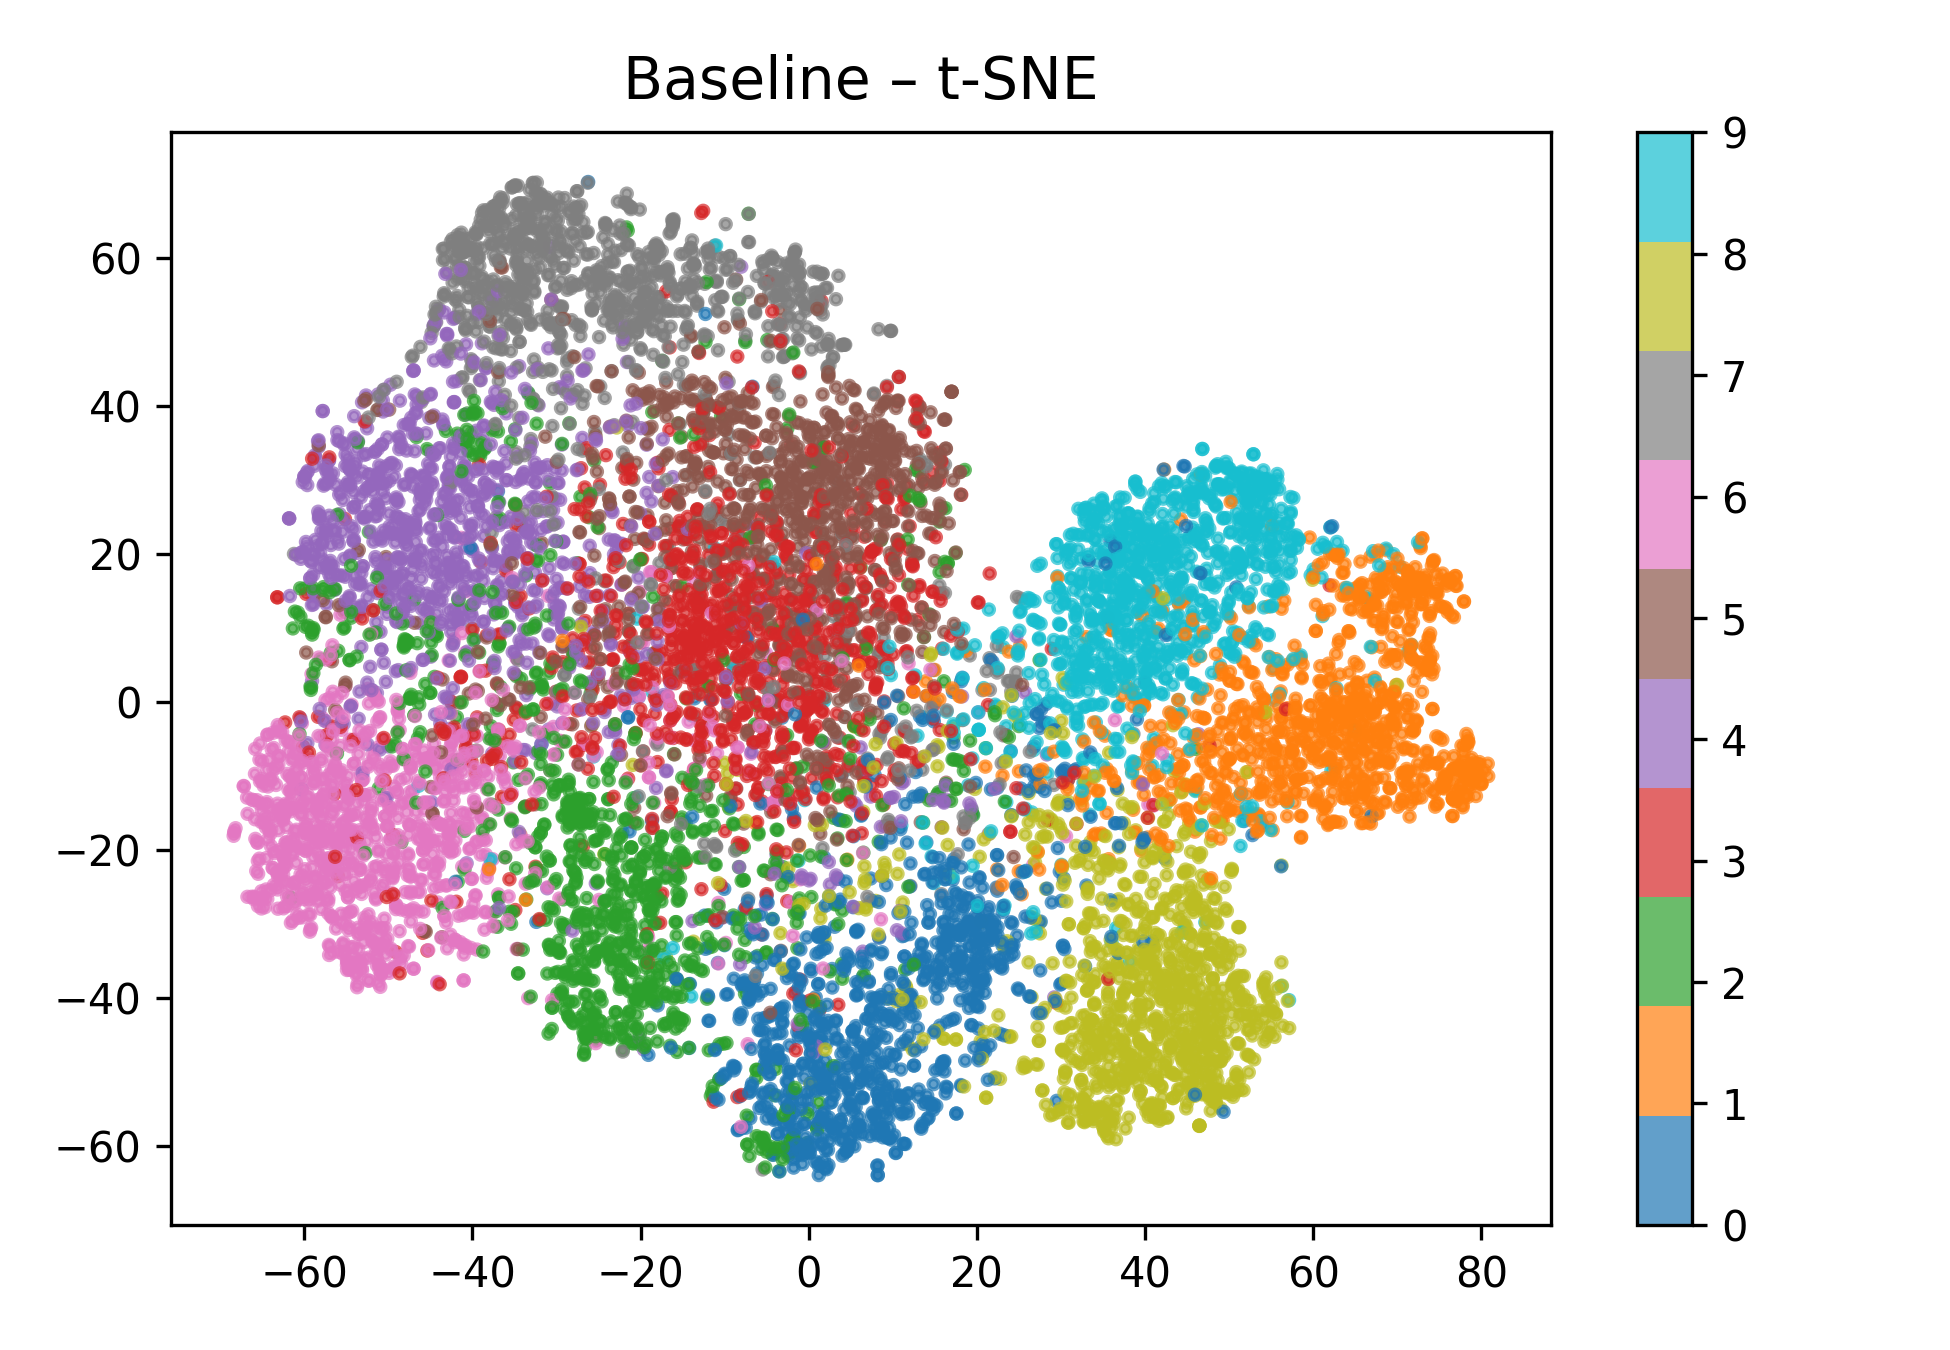
\includegraphics[width=0.9\columnwidth]{picture/baseline_tsne.png}
  }%
  \\[0.3cm] % 强制换行，实现竖向排列
  % 子图 (b)
  \subfloat[With \textit{DenoiseRep\textsuperscript{++}}\label{fig:tsne_denoise}]{
    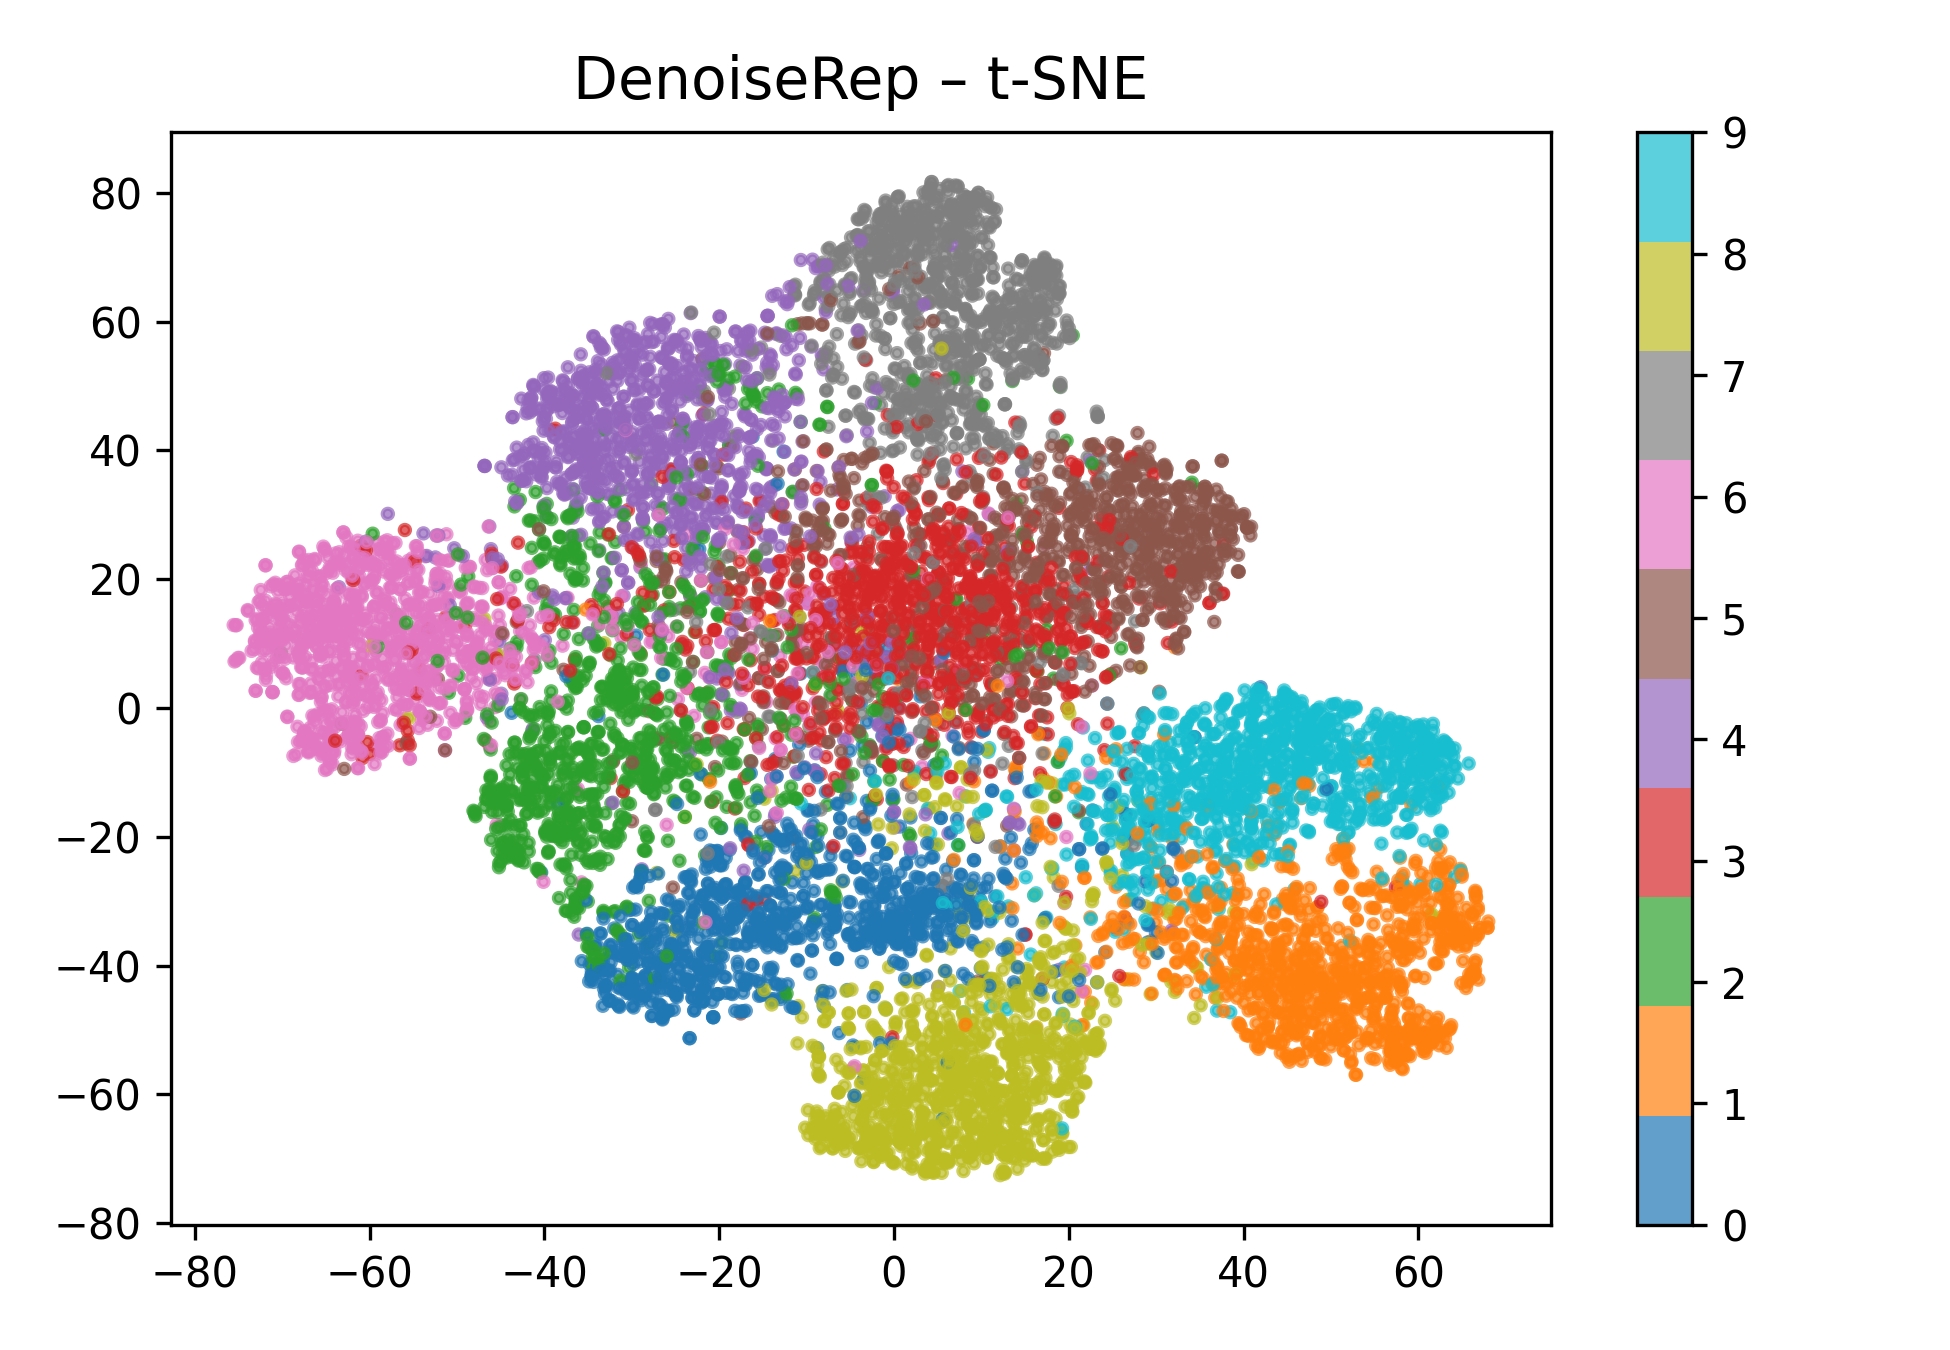
\includegraphics[width=0.9\columnwidth]{picture/denoise_tsne.png}
  }

  \caption{t-SNE visualization of \texttt{[CLS]} token features on cifar-10 classification.
  (a) Baseline. (b) With \textit{DenoiseRep\textsuperscript{++}}.}
  \label{fig:tsne_cls}
\end{figure}

\begin{figure}[t]
    \centering
    
    % 子图 (a) Baseline
    \subfloat[Baseline\label{fig:distance_hist_baseline}]{
        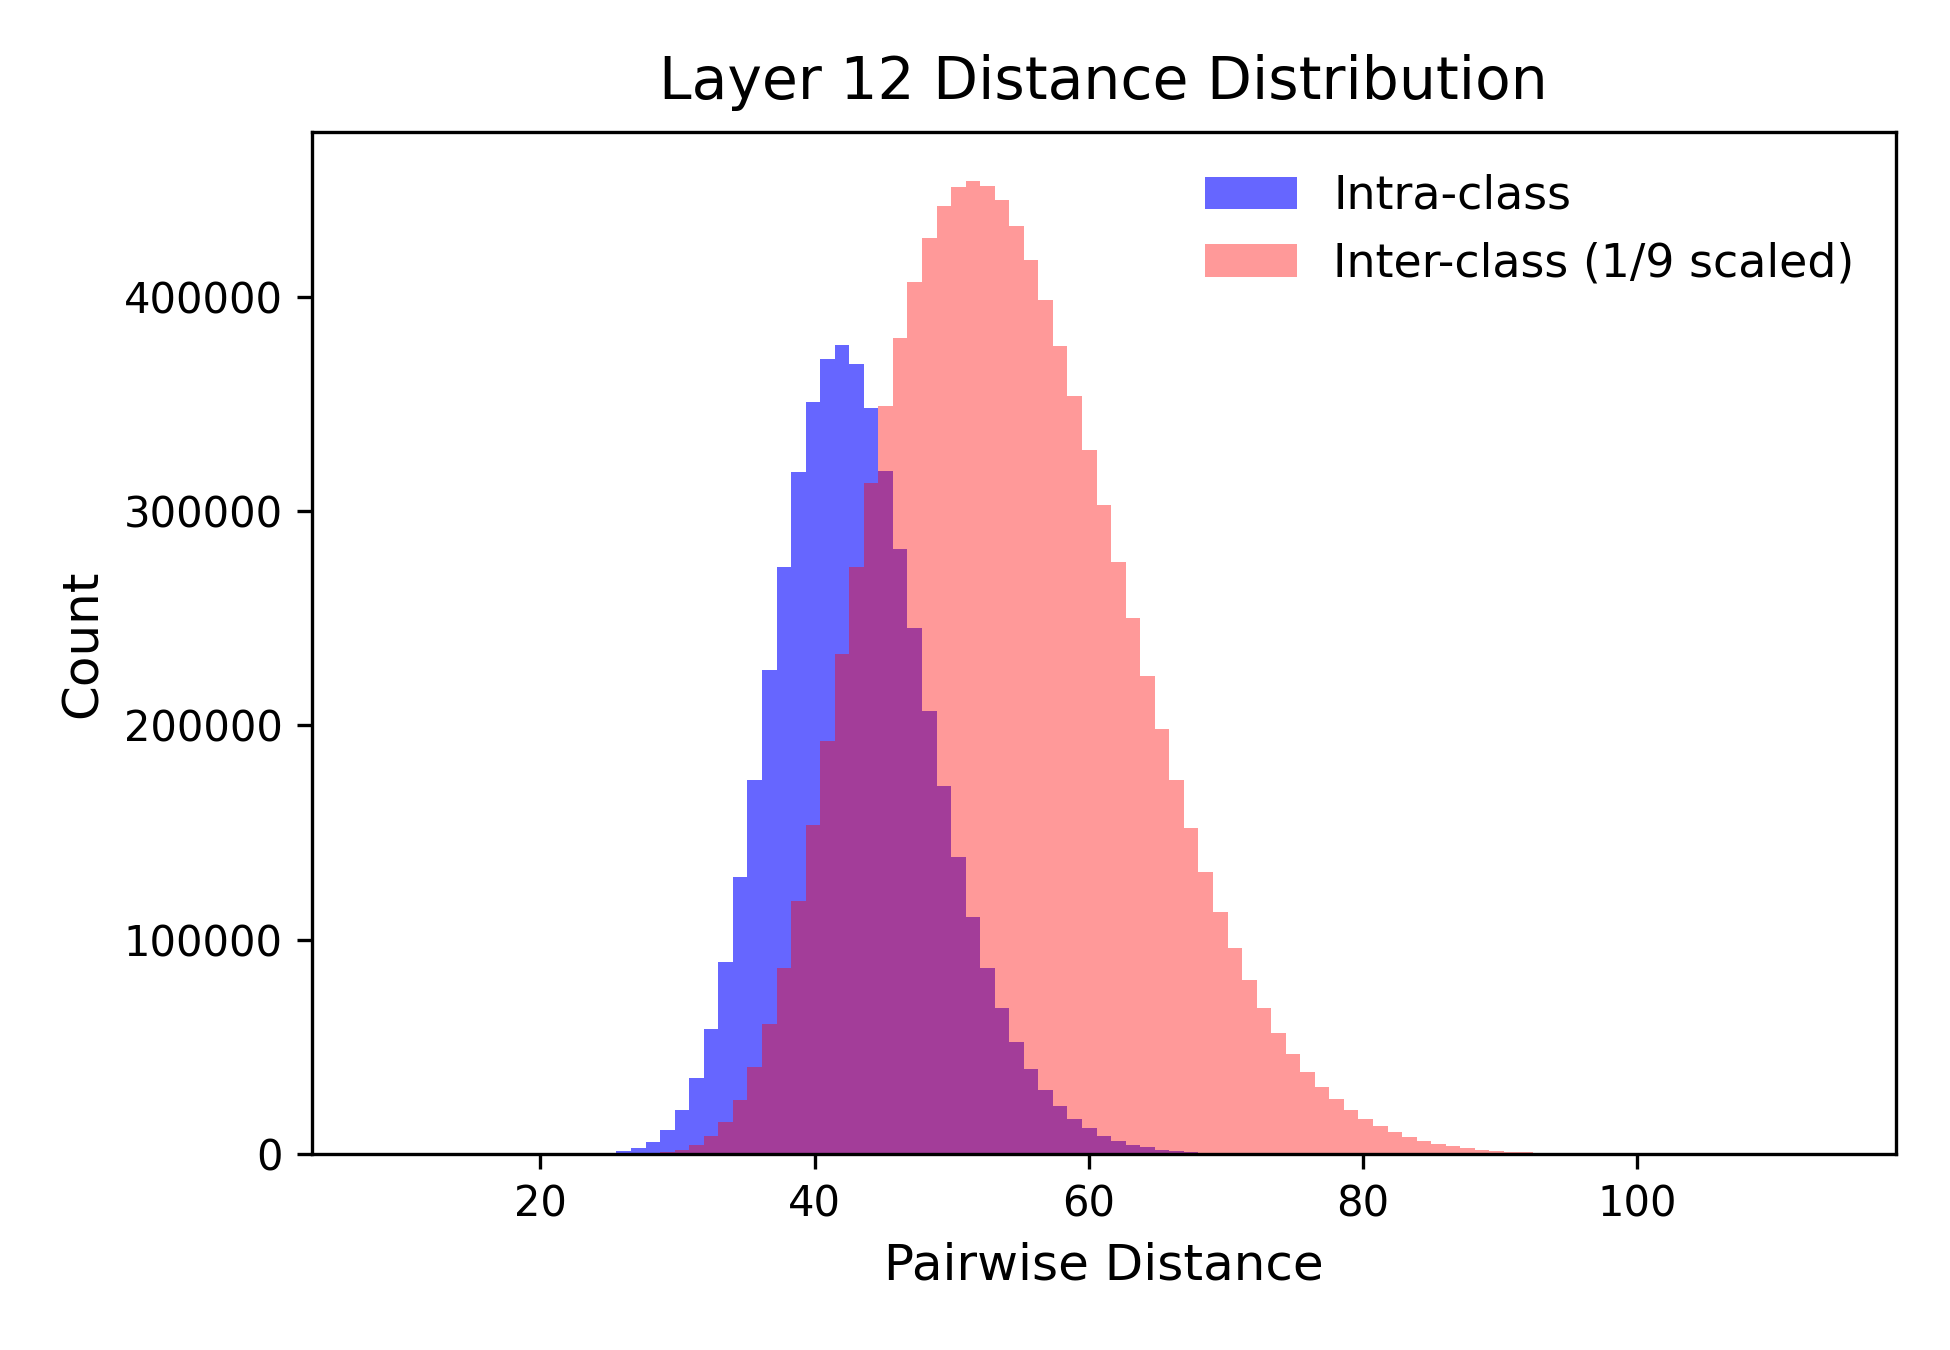
\includegraphics[width=0.8\columnwidth]{picture/layer12_modelA.png}
    }%
    \\[0.3cm] % 强制换行，让两张图竖向排列
    % 子图 (b) With DenoiseRep
    \subfloat[With \textit{DenoiseRep\textsuperscript{++}}\label{fig:distance_hist_denoise}]{
        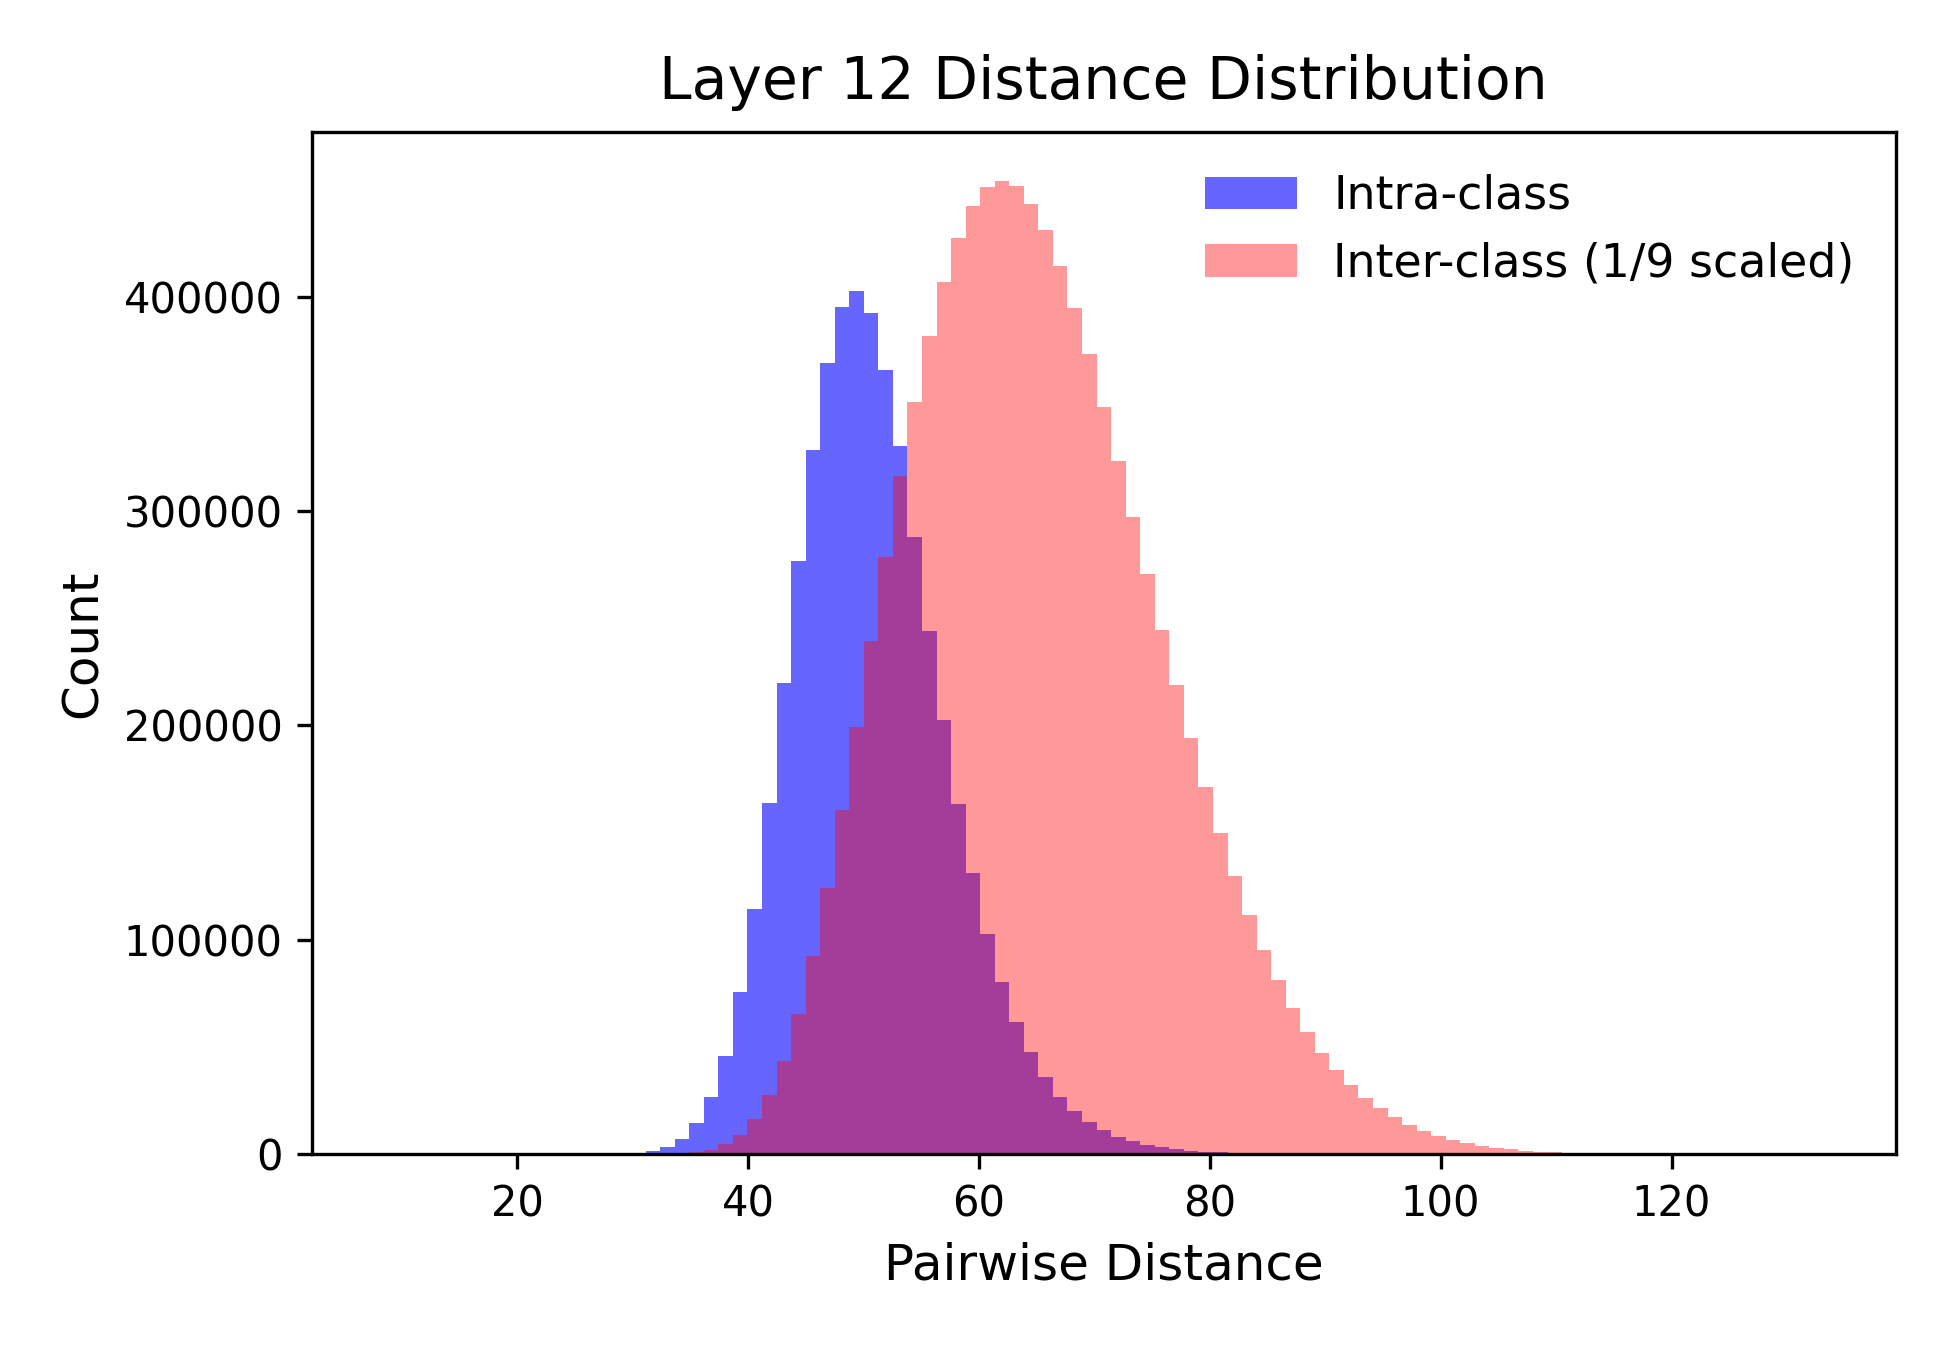
\includegraphics[width=0.8\columnwidth]{picture/layer12_modelB.png}
    }

    \caption{Histogram comparison of intra-class and inter-class distances.
    (a) Baseline model. 
    (b) With \textit{DenoiseRep\textsuperscript{++}}. 
    Denoising reduces the overlap area between intra- and inter-class distributions, indicating improved separability.}
    \label{fig:distance_hist}
\end{figure}

\textbf{Intra- and inter-class distance statistics.} 
To quantitatively validate the above observation, we compute several distance-based statistics:
\begin{itemize}
    \item \textbf{Intra-class distance.} For each category, we calculate the average pairwise Euclidean distance among all features. The global intra-class mean is normalized to 1 for fair comparison, and the variance is reported to measure consistency across classes. 
    \item \textbf{Inter-class distance.} We calculate the average pairwise distances between class centroids, and also compute the variance across different class pairs. 
    \item \textbf{Inter/Intra ratio.} The ratio between inter-class mean and intra-class mean reflects feature separability: higher values indicate stronger discriminability.
    \item \textbf{Histogram overlap.} We estimate the overlap area between intra- and inter-class distance distributions. Smaller overlap implies better separation between categories.
\end{itemize}

\begin{figure*}[t]
    \centering
    
    % =============================================
    % 第一排：Baseline
    % =============================================
    % 左侧文字标签 (占用 3% 宽度)
    \begin{minipage}{0.03\linewidth}
        \centering
        % rotatebox 需要 graphicx 宏包，90度旋转文字
        \rotatebox{90}{\textbf{\textit{Baseline}}} 
    \end{minipage}%
    \hfill
    % 右侧图片组 (占用 96% 宽度)
    \begin{minipage}{0.96\linewidth}
        \centering
        % 既然在 minipage 里，0.19 \linewidth 大约就是 1/5 的宽度
        % 最后的 \hfill 确保图片均匀分布
        \subfloat[]{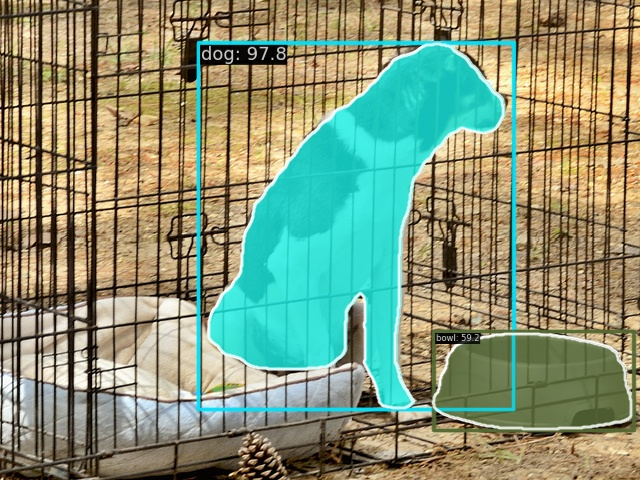
\includegraphics[width=0.19\linewidth]{picture/det_vis/base_01.jpg}}\hfill
        \subfloat[]{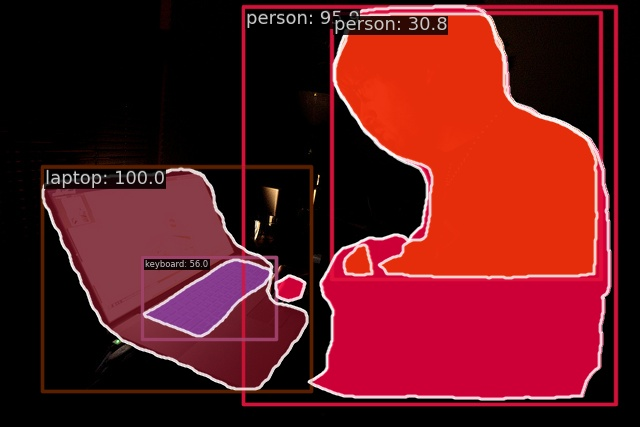
\includegraphics[width=0.19\linewidth]{picture/det_vis/base_03.jpg}}\hfill
        \subfloat[]{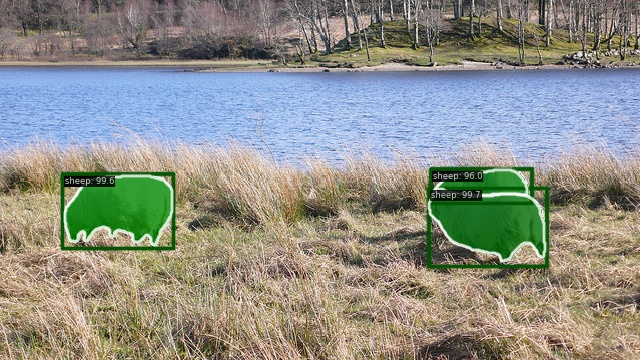
\includegraphics[width=0.19\linewidth]{picture/det_vis/base_04.jpg}}\hfill
        \subfloat[]{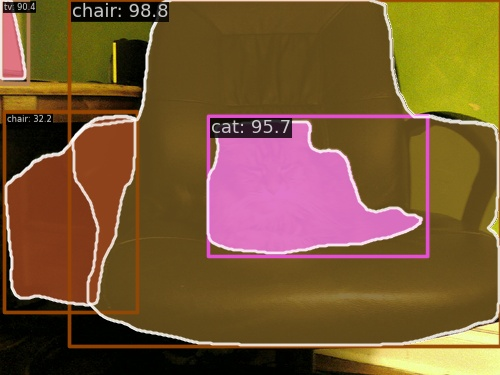
\includegraphics[width=0.19\linewidth]{picture/det_vis/base_05.jpg}}\hfill
        \subfloat[]{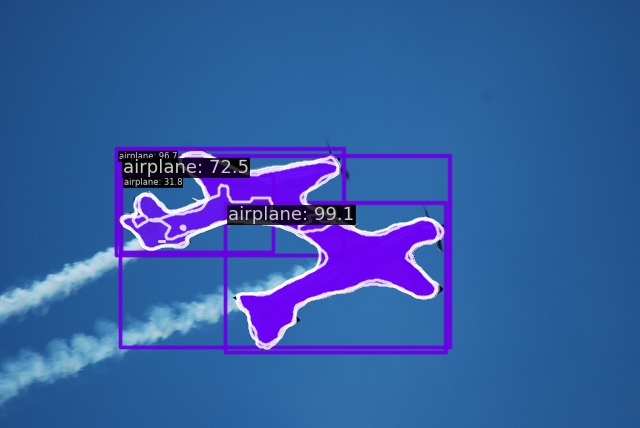
\includegraphics[width=0.19\linewidth]{picture/det_vis/base_06.jpg}}
    \end{minipage}

    \vspace{2mm} % 两排之间的间距

    % =============================================
    % 第二排：DenoiseRep (Ours)
    % =============================================
    % 左侧文字标签
    \begin{minipage}{0.03\linewidth}
        \centering
        \rotatebox{90}{\textbf{\textit{DenoiseRep\textsuperscript{++}}}} % 或者写 Ours
    \end{minipage}%
    \hfill
    % 右侧图片组
    \begin{minipage}{0.96\linewidth}
        \centering
        \subfloat[]{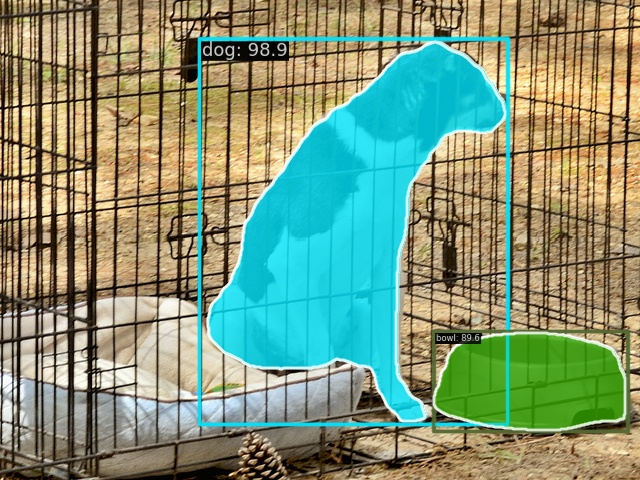
\includegraphics[width=0.19\linewidth]{picture/det_vis/denoiserep_01.jpg}}\hfill
        \subfloat[]{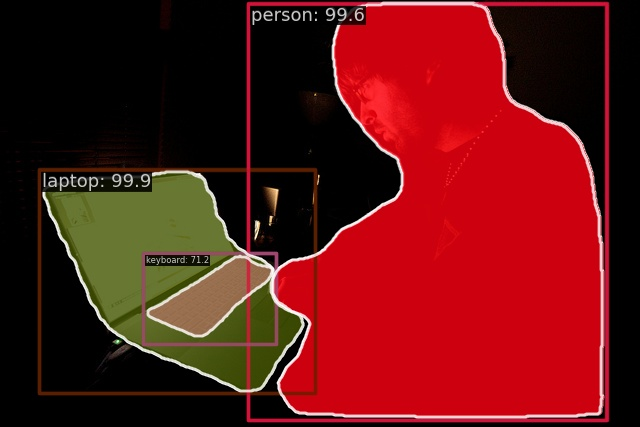
\includegraphics[width=0.19\linewidth]{picture/det_vis/denoiserep_03.jpg}}\hfill
        \subfloat[]{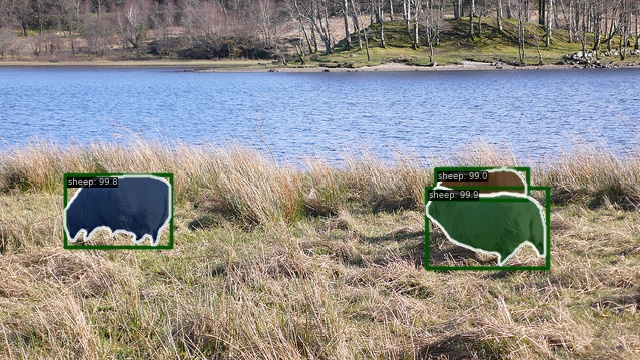
\includegraphics[width=0.19\linewidth]{picture/det_vis/denoiserep_04.jpg}}\hfill
        \subfloat[]{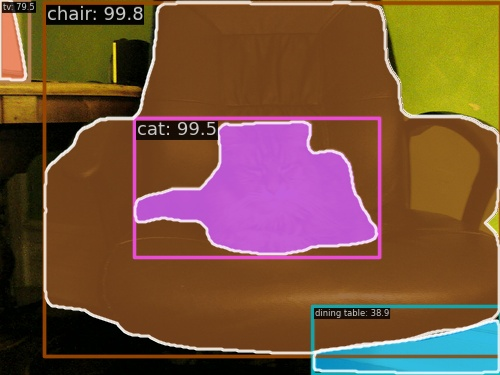
\includegraphics[width=0.19\linewidth]{picture/det_vis/denoiserep_05.jpg}}\hfill
        \subfloat[]{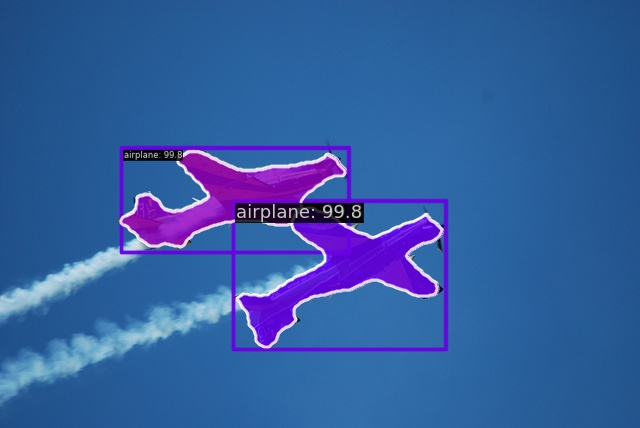
\includegraphics[width=0.19\linewidth]{picture/det_vis/denoiserep_06.jpg}}
    \end{minipage}

    \caption{Qualitative comparison of object detection results.
    (a)-(e) Results of the Baseline model. 
    (f)-(j) Results of the proposed \textit{DenoiseRep\textsuperscript{++}}.
    The visual comparison demonstrates that our method effectively reduces false positives and improves bounding box precision.}
    \label{fig:qualitative_denoiserep}
\end{figure*}


\begin{figure*}[t]
    \centering
    
    % =============================================
    % 第一行：Baseline
    % =============================================
    % 1. 左侧文字标签 (占用约 3% 宽度)
    \begin{minipage}{0.03\linewidth}
        \centering
        \rotatebox{90}{\textbf{\textit{Baseline}}}
    \end{minipage}%
    \hfill
    % 2. 右侧图片 (占用约 96% 宽度)
    \begin{minipage}{0.96\linewidth}
        \centering
        % 让图片占满这个 minipage 的宽度
        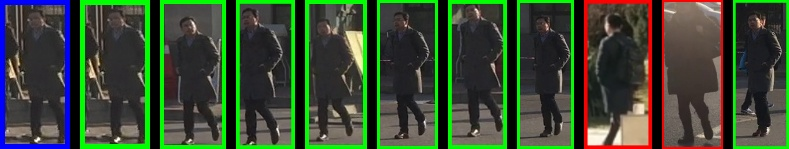
\includegraphics[width=\linewidth]{picture/reid_vis/reid_base.jpg}
    \end{minipage}

    \vspace{2mm} % 上下行间距

    % =============================================
    % 第二行：Ours (DenoiseRep++)
    % =============================================
    \begin{minipage}{0.03\linewidth}
        \centering
        % 这里文字较长，可能需要微调字体大小，或者简写为 Ours
        \rotatebox{90}{\textbf{\textit{DenoiseRep\textsuperscript{++}}}} 
    \end{minipage}%
    \hfill
    \begin{minipage}{0.96\linewidth}
        \centering
        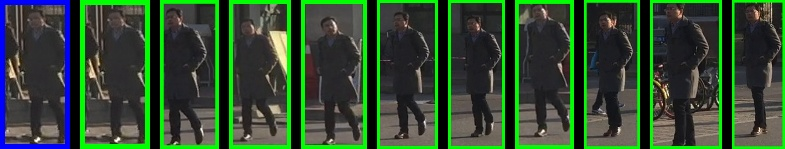
\includegraphics[width=\linewidth]{picture/reid_vis/reid_denoise.jpg}
    \end{minipage}

    % =============================================
    % 丰富的 Caption
    % =============================================
    \caption{Qualitative visualization of person re-identification ranking results. 
    The left-most image in each row represents the \textbf{query}, followed by the top-ranked retrieved images from the gallery.
    (Top) The Baseline model is easily distracted by background clutter or noise, leading to incorrect matches (false positives). 
    (Bottom) Armed with our \textit{DenoiseRep\textsuperscript{++}}, the model extracts more robust and discriminative features, significantly improving retrieval accuracy and ranking quality.}
    \label{fig:reid_vis_vertical}
\end{figure*}

\textbf{Statistical results.} 
Table~\ref{tab:distance_stats} summarizes the statistics before and after denoising. Compared with the baseline, the denoised features show: (1) lower intra-class variance, meaning features within the same category are more consistent; (2) higher inter-class mean, suggesting that categories are further apart; and (3) an improved inter/intra ratio, indicating better overall separability. Furthermore, the histogram overlap decreases after denoising, confirming that the distributions of intra- and inter-class distances are better separated. 


\begin{table}[htbp!]
\centering
\caption{Statistical analysis of intra-class and inter-class distances on cifar-10 validation set. Intra-class mean is normalized to 1.}
\label{tab:distance_stats}
\vspace{0.2cm}
\renewcommand{\arraystretch}{1.2}
\begin{tabular}{l|c|c}
\hline \hline
\textbf{Metric} & \textbf{Baseline} & \textbf{+DenoiseRep\textsuperscript{++}} \\
\hline
Intra Var      & 0.019 & 0.017 \\
Inter Mean     & 43.096 & 50.755 \\
Inter Var      & 54.132 & 64.959 \\
Inter/Intra    & 1.256 & 1.280 \\
Overlap        & 0.463 & 0.4161 \\
\hline \hline
\end{tabular}
\end{table}


\begin{figure*}[t]
    \centering
    \subfloat[Example 1: Pearson $r{=}0.827$, Att-IoU@0.5${=}0.521$]{%
        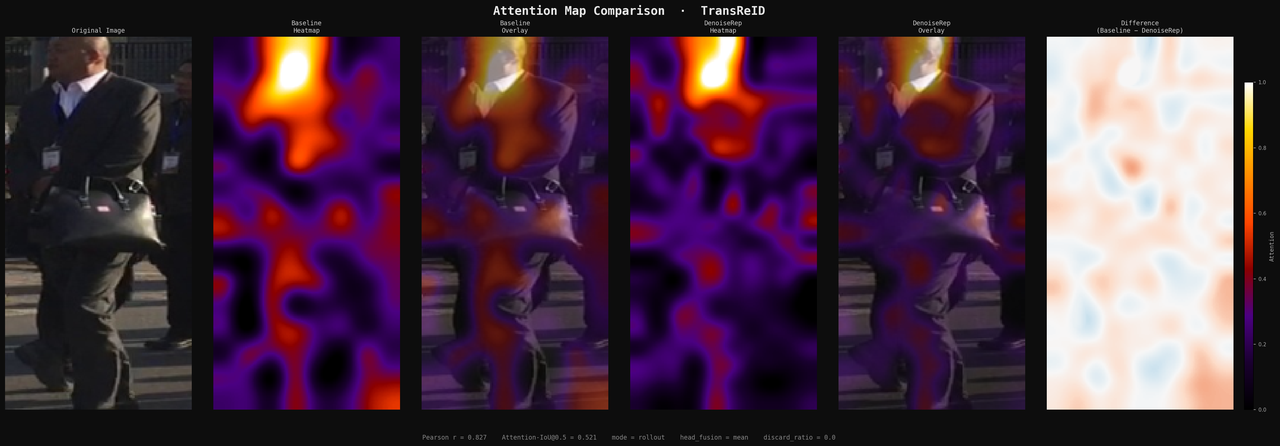
\includegraphics[width=0.48\textwidth]{picture/attn_reid_1.png}%
    }\hfill
    \subfloat[Example 2: Pearson $r{=}0.811$, Att-IoU@0.5${=}0.537$]{%
        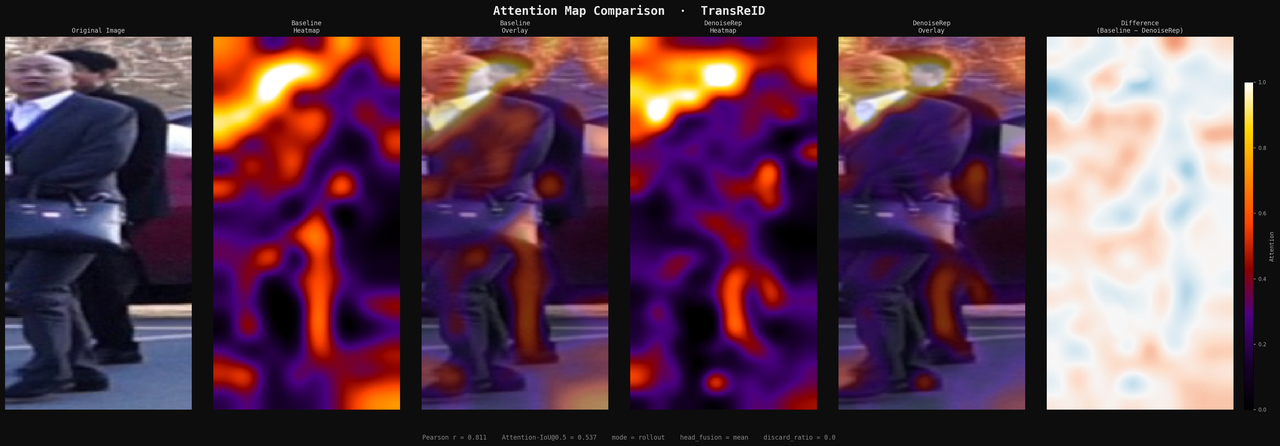
\includegraphics[width=0.48\textwidth]{picture/attn_reid_2.png}%
    }%
    \\[1ex]
    \subfloat[Example 3: Pearson $r{=}0.641$, Att-IoU@0.5${=}0.489$]{%
        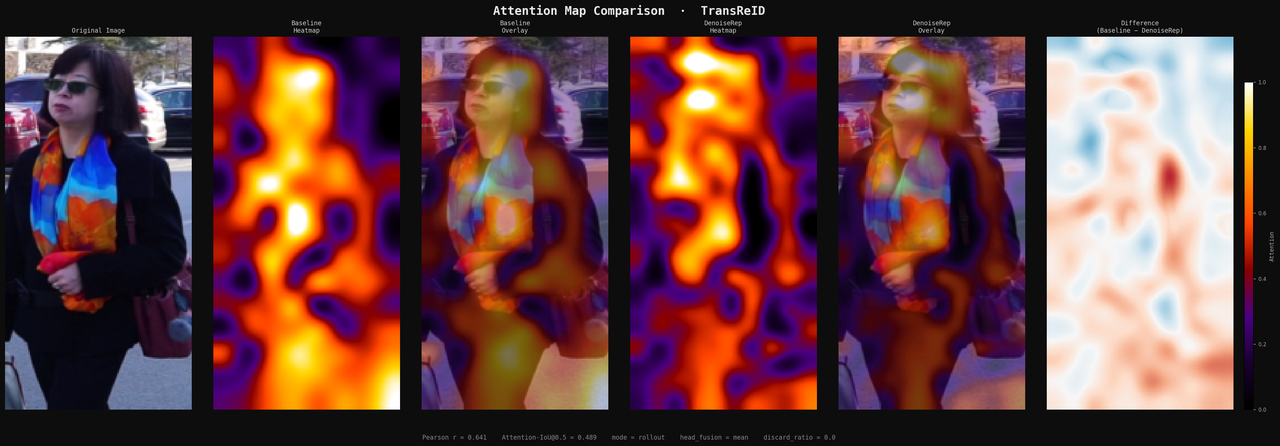
\includegraphics[width=0.48\textwidth]{picture/attn_reid_3.png}%
    }\hfill
    \subfloat[Example 4]{%
        
\includegraphics[width=0.48\textwidth]{picture/attn_reid_4.png}%
    }
    \caption{Attention map comparison between the Baseline and \textit{DenoiseRep\textsuperscript{++}} on person re-identification (DukeMTMC-reID). Each sub-figure shows, from left to right: original image, baseline attention heatmap, baseline overlay, \textit{DenoiseRep\textsuperscript{++}} heatmap, \textit{DenoiseRep\textsuperscript{++}} overlay, and the pixel-wise difference map (Baseline $-$ \textit{DenoiseRep\textsuperscript{++}}). After denoising, the model's attention is more concentrated on identity-discriminative regions (e.g., face, clothing) and less responsive to background distractors.}
    \label{fig:attn_map_reid}
\end{figure*}

\textbf{Discussion.} 
Both the qualitative (t-SNE) and quantitative (statistical measures) analyses lead to consistent conclusions: 
(1) \textit{DenoiseRep\textsuperscript{++}} reduces intra-class variability, making features more compact; 
(2) it enlarges inter-class margins, yielding clearer class separation; 
(3) the overall distribution overlap between intra- and inter-class distances is reduced, confirming improved feature quality. 
Together, these analyses provide strong evidence that denoising at the feature level improves not only classification accuracy but also the underlying representation geometry, which is critical for downstream discriminative tasks.


\textbf{Qualitative Analysis on Downstream Tasks.} 
Beyond image classification, we qualitatively verify the generalization capability of our method on dense prediction and retrieval tasks. 
Fig.~\ref{fig:qualitative_denoiserep} illustrates the comparison for object detection and instance segmentation. 
As shown in the top row, the Baseline model tends to generate false positives and inaccurate segmentation boundaries, particularly in ambiguous or cluttered regions (e.g., the extra artifacts in Fig.~\ref{fig:qualitative_denoiserep}(d)). 
In contrast, \textit{DenoiseRep\textsuperscript{++}} (bottom row) effectively suppresses these noise-induced artifacts, yielding tighter bounding boxes and more precise masks. 
Furthermore, Fig.~\ref{fig:reid_vis_vertical} visualizes the retrieval ranking results for person re-identification. 
While the Baseline model is prone to retrieving incorrect identities (marked with red borders) due to background distractions or similar clothing, our method consistently retrieves correct matches (marked with green borders) in the top ranks. 
These visualizations confirm that the proposed feature denoising strategy significantly enhances representation robustness, reducing the impact of task-irrelevant noise in both detection and retrieval scenarios.


\textbf{Attention map interpretability analysis.}
To provide an interpretable understanding of how feature-level denoising affects model behavior, we visualize the attention maps of the baseline and \textit{DenoiseRep\textsuperscript{++}} models on the person re-identification task. Specifically, we employ Attention Rollout~\cite{abnar2020quantifying} to aggregate multi-head attention across all transformer layers with mean fusion, generating holistic attention heatmaps for each input image.

As shown in Fig.~\ref{fig:attn_map_reid}, we present three representative examples from the DukeMTMC-reID dataset. For each example, we visualize the original image, baseline attention heatmap and overlay, \textit{DenoiseRep\textsuperscript{++}} attention heatmap and overlay, and their pixel-wise difference map. Several key observations emerge:

(1) \textit{The denoised model focuses more on identity-discriminative regions.} Comparing the heatmaps of the baseline and \textit{DenoiseRep\textsuperscript{++}}, the denoised model concentrates attention more on semantically meaningful body regions—such as the face, upper body, and clothing textures—that are critical for identity discrimination. In contrast, the baseline model distributes attention more diffusely, including background regions and other non-informative areas.

(2) \textit{Environmental noise receives less attention after denoising.} The difference maps (rightmost column) clearly illustrate that \textit{DenoiseRep\textsuperscript{++}} reduces attention on background elements such as other pedestrians, street furniture, and cluttered surroundings. The warm-colored regions (positive difference) in the difference map indicate areas where the baseline allocates more attention than the denoised model, which predominantly correspond to background distractors.

(3) \textit{Quantitative attention metrics confirm the improvement.} We compute the Pearson correlation coefficient between the attention map and the person bounding box mask, as well as Attention-IoU@0.5 (the IoU between the thresholded attention region and the ground-truth person region). The Pearson $r$ values range from 0.641 to 0.827, and Attention-IoU@0.5 values range from 0.489 to 0.537, indicating that the attention redistribution is nuanced rather than trivially concentrated, reflecting a refined, identity-aware focus rather than simple spatial localization.

These results provide interpretable evidence that feature-level denoising effectively suppresses the model's response to task-irrelevant noise, redirecting attention towards discriminative identity cues. This mechanism explains why \textit{DenoiseRep\textsuperscript{++}} achieves improved performance across retrieval and recognition tasks: by denoising the intermediate features, the model learns to attend to the most informative regions while being less distracted by environmental interference.


\subsection{Fairness Experiment}
To ensure the fairness of the experiment, we compared the performance of the baseline method with our proposed method under the same conditions. Specifically, during the training process, we strictly controlled the experimental variables so that both the baseline method and our method ran under the same number of training epochs and hyperparameter settings. 

\begin{table}[htbp]
\centering
\caption{Comparison of performance between baseline method and our proposed method in the same additional training epochs. The baseline method TransReID-SSL is based on ViT-small backbone.}
\label{tab:Fairness Experiment}
\vspace{0.2cm}
\renewcommand{\arraystretch}{1.2}
\begin{tabular}{lcccc} % 不加竖线，内容更紧凑
\hline \hline
\textbf{Epoch} & \textbf{120} & \textbf{160} & \textbf{200} & \textbf{240} \\ 
\midrule
Baseline & 81.18\% & 81.19\% & 81.18\% & 81.16\% \\
+\textit{DenoiseRep} & 81.18\% & 81.64\% & 82.00\% & 82.12\% \\
\hline \hline
\end{tabular}
\end{table}

The experimental results in Table \ref{tab:Fairness Experiment} indicate that the baseline method did not show significant performance improvement under the same number of training epochs. This observation indicates that the performance improvement obtained is attributed to our proposed method, rather than an increase in training time or number of epochs, which validates the effectiveness of our method.

\section{Conclusion}


In this work, we have presented \textit{DenoiseRep\textsuperscript{++}}, a novel framework that effectively bridges the gap between generative diffusion models and discriminative representation learning. By reinterpreting the backbone network as a recursive denoising process, we demonstrate that generative denoising objectives can significantly enhance feature separability and robustness without requiring ground-truth labels.
A key innovation of our approach lies in achieving these gains with zero additional inference latency via parameter fusion. To overcome the inherent capacity limitations of lightweight denoising modules, we introduced two synergistic enhancements: (1) a Teacher-Student Distillation framework that utilizes a high-capacity teacher to calibrate the denoising direction and reduce estimation bias; and (2) a Multi-step Fusion strategy that simulates a progressive denoising trajectory, thereby mitigating discretization errors associated with single-step inference. Extensive experiments across image classification, object detection, segmentation, and person re-identification validate that \textit{DenoiseRep\textsuperscript{++}} consistently minimizes intra-class variance and maximizes inter-class margins.
Future Work. \textit{DenoiseRep\textsuperscript{++}} establishes a generalizable, model-agnostic paradigm. Future directions include extending this mechanism to multi-modal frameworks (e.g., CLIP) to enhance cross-modal alignment, and applying it to video understanding to handle temporal noise. Furthermore, while our current approach relies on linear parameter fusion, exploring non-linear approximation techniques inspired by Flow Matching or ODE solvers could offer new avenues for integrating even more complex generative priors into discriminative backbones efficiently.

\section*{Acknowledgment}

This work was supported in part by the National Key Research and Development Program of China under Grant (2023YFC3310700), the National Natural Science Foundation of China (62572040, 62202041), the Beijing Natural Science Foundation (JQ24019), and the Fundamental Research Funds for the Central Universities (2025JBMC011).

\bibliographystyle{plainnat}
\bibliography{reference}

\end{document}
